\apendice{Especificación de diseño}

\section{Introducción}
Este apartado trata de recoger y explicar todos los elementos que construyen la estructura y diseño de la aplicación y cómo se relacionan entre sí para satisfacer los requisitos expuestos en el apartado anterior.

Hay que destacar que el espectro de datos que utiliza la aplicación abarca más que su código, ya que, al ser un proyecto multidisciplinar, integra datos de distintos tipos, como pistas de audio, modelos 3D, interfaces, texturas o animaciones.

Por tanto, el diseño de estos datos se debe tener en cuenta en el análisis general de la aplicación. 

\section{Diseño de datos} 
\subsection{Guardado y carga de datos}
Para dotar al proyecto de funcionalidades de carga y guardado de datos, se ha integrado la base de datos \textbf{\textit{Realtime Database de FireBase}}.\\
Se trata de una base de datos NoSQL alojada en la nube que tiene una sencilla integración con Unity y que permite almacenar y sincronizar los datos entre los usuarios en tiempo real, siendo accesibles incluso sin conexión \cite{wiki:Firebase}.

En este caso, se pretende construir una base de datos sencilla que almacene de cada jugador su \textbf{nombre de usuario} y su \textbf{experiencia total}.

Las bases de datos NoSQL como la utilizada en este proyecto almacenan los datos en formato JSON, y no en forma de tablas. Por lo tanto, la estructura de datos de la aplicación se vería como en la figura \ref{fig:EstructuraJSON}, en la que en ese momento habría dos usuarios registrados en la aplicación.
\begin{figure}[h]
	\centering
	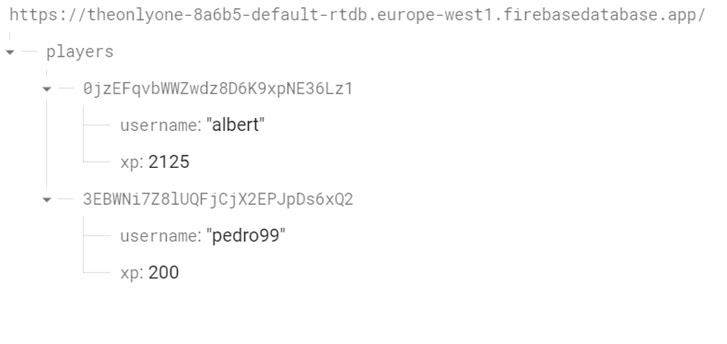
\includegraphics[scale=0.45]{img/DatabaseNoSQL.jpg}
	\caption{Datos almacenados en formato JSON}
	\label{fig:EstructuraJSON}
    \end{figure}
Para que el acceso de lectura y escritura de la base de datos esté restringido y por tanto protegido, todos los usuarios de la aplicación deben identificarse.

Gracias a \textbf{\textit{Firebase Authentication}}, se pueden definir de manera sencilla qué método de autenticación tendrá la aplicación. Para este proyecto se ha utilizado un procedimiento mediante el cual cada usuario debe proporcionar un correo y una contraseña para poder acceder a su cuenta.

Además, para garantizar la seguridad en la base de datos, Firebase proporciona reglas de seguridad para determinar quién puede acceder y/o modificar qué datos, y cómo se estructuran los datos.
Las reglas definidas en la aplicación son:
\begin{enumerate}
    \item Solamente los usuarios autenticados pueden leer los datos de los demás usuarios.
    \item Un usuario solamente puede escribir sus propios datos y no los de los demás usuarios.
\end{enumerate}
Cuando un usuario nuevo se registra en la aplicación, la clase FireBaseManager crea una nueva entrada en la base de datos asociada a al jugador, junto a un identificador único asignado por el propio gestor, el nombre de usuario que eligió al registrarse y la experiencia (xp) inicial vacía (0). 

Cuando este jugador inicie sesión, la base de datos ya lo tendrá localizado, permitiéndole ir al menú principal, donde verá su nombre de usuario y su experiencia actual. 
Además de sus propios datos, también podrá ver los datos de los jugadores con más experiencia del juego accediendo al apartado ``clasificación'', donde se muestran sus nombres de usuario y sus respectivas experiencias. Al momento de pulsar dicho botón, la clase \textit{GetUsersData} hace una petición de consulta a la base de datos para recuperar los datos de los mejores jugadores del videojuego, en orden de mayor a menor. Entonces, el videojuego crea una fila visual para cada jugador con su información para ser mostrada en la clasificación.

Para que el usuario pueda aumentar su experiencia, deberá completar partidas, y dependiendo de su desempeño en ellas, ganará más o menos experiencia. Al terminar una partida, la clase \textit{GameManager} enviará una petición de escritura a la base de datos para modificar el atributo correspondiente a la experiencia del usuario, sumándole la ganada en dicha partida.
Concretamente, se utiliza la función \textbf{\textit{SetValueAsync()}} para escribir y actualizar algún atributo específico, y \textbf{\textit{GetValueAsync()}} para obtener una instantánea estática del contenido de la ruta especificada que contendrá todos los datos pedidos, a partir de la cual se extraen los datos deseados.
El flujo de datos entre la aplicación y la base de datos se puede visualizar de manera esquematizada en la figura \ref{fig:EsquemaBBDD}:
\begin{figure}[h]
	\centering
	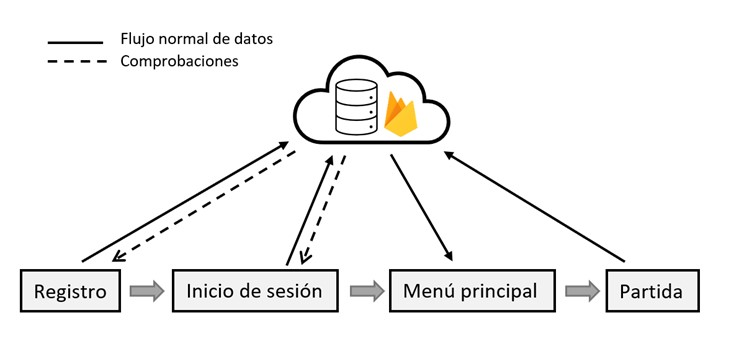
\includegraphics[scale=0.45]{img/DataFlowDiagram.jpg}
	\caption{Esquema del flujo de datos con la base de datos}
	\label{fig:EsquemaBBDD}
    \end{figure}
\subsection{Managers}
A la hora de definir la jerarquía de clases del proyecto, existen algunas clases que se definen como Managers o Gestores de las demás. Estas actúan como controladores de diferentes secciones del videojuego, centralizando varios elementos y asegurándose de que todo funciona como se espera. En este proyecto, existen algunas clases a destacar de este estilo, que suelen ser referenciadas de manera recurrente por el resto de clases.

La clase \textbf{\textit{SceneDirector}} (ver figura \ref{fig:SceneDirector}) es la responsable del manejo de escenas de la aplicación. Cada vez que se desea cambiar de escena se debe llamar a esta clase, y en concreto a su método \textit{LoadScene(escena)}, que internamente hará lo necesario para cargar la escena objetivo de forma consistente, mostrando una pantalla de carga durante el proceso. También será la clase llamada cuando se quiera cerrar la aplicación, con el método \textit{QuitGame()}.

\begin{figure}[h]
	\centering
	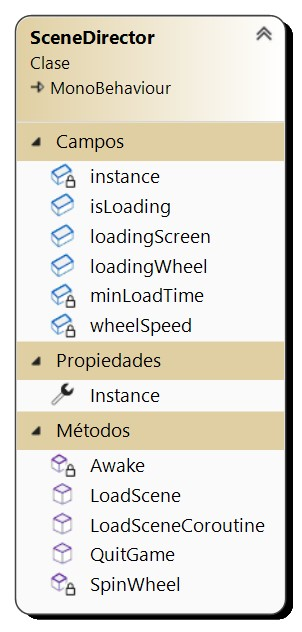
\includegraphics[scale=0.45]{img/SceneDirector.jpg}
	\caption{Clase \textit{SceneDirector}}
	\label{fig:SceneDirector}
    \end{figure}

\textbf{\textit{AudioManager}} (ver figura \ref{fig:AudioManager}) es la clase encargada de gestionar gran parte de los sonidos generales del videojuego, como los relacionados con la música, los botones de las interfaces, y todos los relativos al jugador, como los efectos sonoros de curarse y recibir daño.
\begin{figure}[h]
	\centering
	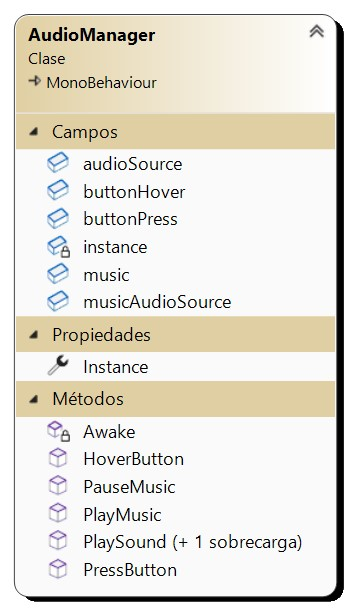
\includegraphics[scale=0.45]{img/AudioManager.jpg}
	\caption{Clase \textit{AudioManager}}
	\label{fig:AudioManager}
    \end{figure}
Ambas clases implementan el patrón de diseño Singleton \cite{wiki:Singleton}, un patrón de diseño creacional que permite asegurar que una clase tiene una única instancia, al tiempo que proporciona un punto de acceso global a dicha instancia. Además, se marcan con el método \textit{DontDestroyOnLoad()} \cite{doc:DontDestroyOnLoad} para que los gameobjects que las contienen no se destruyan al cambiar de escena y así poder acceder a ellos y, por tanto, a las clases desde cualquier escena. Esto es importante para mantener la consistencia de datos a través de toda la aplicación y evitar errores asociados a la duplicidad o ambigüedad de elementos.\\
Por ejemplo, si el objeto que contiene a la clase \textit{AudioManager} se destruyese al cambiar de una escena a otra, la música que pueda estar sonando se pararía y volvería a comenzar de nuevo. Esto se evita con las técnicas descritas, pudiendo tener un hilo de música continuo en toda la aplicación.

La clase \textbf{\textit{ButtonsManager}} (ver figura \ref{fig:ButtonsManager}) tiene como objetivo centralizar y gestionar el comportamiento de todos los botones presentes en la aplicación, para, de esta forma, tenerlos más organizados y que puedan ser modificados y administrados más fácilmente. En este caso no se requiere mantener una única referencia de esta clase en toda la aplicación, ya que cada escena la utilizará unos atributos distintos en función de la escena actual, a diferencia de las dos clases anteriores, cuyos atributos son consistentes en todo el sistema.
\begin{figure}[h]
	\centering
	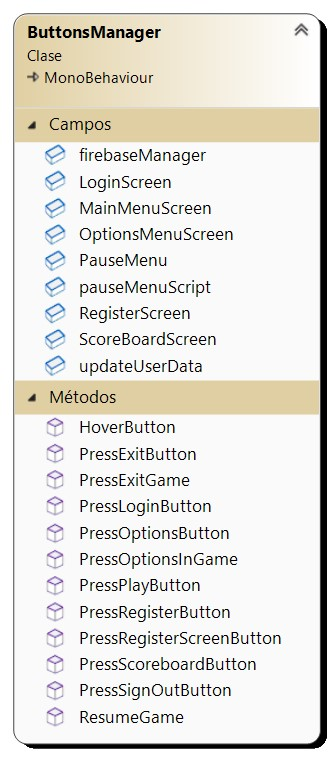
\includegraphics[scale=0.45]{img/ButtonsManager.jpg}
	\caption{Clase \textit{ButtonsManager}}
	\label{fig:ButtonsManager}
    \end{figure}
Además de la autenticación, \textbf{\textit{FirebaseManager()}} (ver figura \ref{fig:FirebaseManager})gestiona todos los aspectos relacionados con la base de datos del videojuego, incluyendo los datos de los usuarios y la consistencia de los mimos. Contiene ciertos atributos estáticos para que sean accesibles en cualquier lugar a nivel de clase, como ``Auth'' (autenticación), ``User''(usuario activo) y ``DBReference'' (base de datos).
\begin{figure}[h]
	\centering
	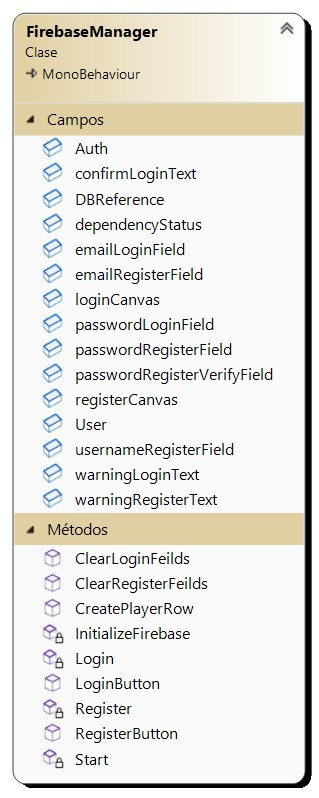
\includegraphics[scale=0.45]{img/FirebaseManager.jpg}
	\caption{Clase \textit{FirebaseManager}}
	\label{fig:FirebaseManager}
    \end{figure}
Por último, una de las clases más importantes en la jerarquía es la clase \textbf{\textit{GameManager}} (ver figura \ref{fig:GameManager}), responsable de que todos los elementos, una vez iniciada la partida, funcionen e interactúen entre ellos adecuadamente para garantizar la correcta ejecución del juego.

Entre sus funciones destacan:
\begin{itemize}
    \item Llevar la cuenta del número de entidades (jugador y enemigos) que siguen vivos, un elemento muy relevante dentro del género battle royale
    \item Actualizar algunos elementos visuales como los enemigos que quedan, los que ha eliminado el jugador o la munición del arma activa, si la hubiere.
    \item Detectar si la partida termina
    \item Determinar el puesto en que queda el jugador al terminar la partida (y si gana o no)
    \item Calcular la experiencia ganada por el jugador durante la partida
    \item Actualizar la experiencia del jugador en la base de datos
    \item Generar las etiquetas flotantes de los objetos de la partida que lo requieran
    \item Mostrar las pantallas de victoria, derrota o estadísticas con la respectiva información
    \item Una de sus funciones principales consiste en convertirse en un lugar centralizado donde definir varios elementos y datos que se utilizarán durante la partida:
    \begin{itemize}
    \item Tipos de armas que pueden existir
    \item Rarezas disponibles de cada arma
    \item Tipos de granadas que pueden existir
    \item Tipos de enemigos que pueden existir
    \item Tipos de packs de ayuda que pueden existir
    \item Rarezas disponibles de cada pack de ayuda
    \item Objetos que se pueden encontrar en las cajas de suministros o que suelten los enemigos al morir
    \end{itemize}
    \item También se definen algunos valores relevantes para la partida, como el radio inicial de la zona segura o cuánta experiencia gana el jugador por cada enemigo eliminado, por completar la partida o por ganarla.
\end{itemize}
\begin{figure}[h]
	\centering
	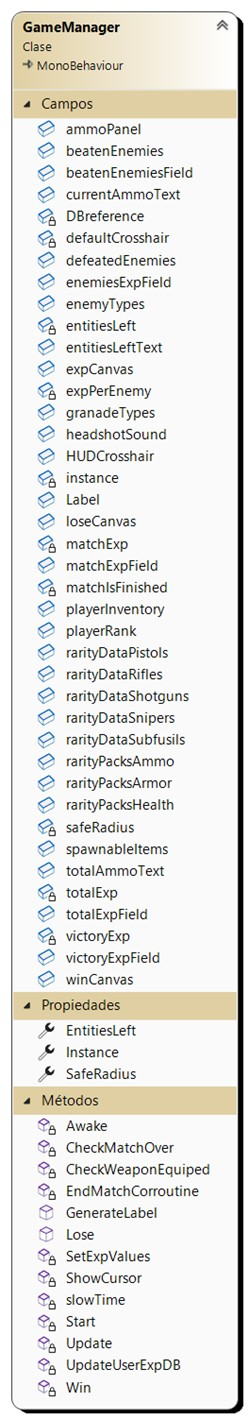
\includegraphics[scale=0.45]{img/GameManager.jpg}
	\caption{Clase \textit{GameManager}}
	\label{fig:GameManager}
    \end{figure}
Otras dos clases a destacar que se encargan de gestionar datos de otras clases son \textbf{\textit{PlayerController}} y \textbf{\textit{EnemyController}} (ver figura \ref{fig:ControladoresJugadorYEnemigo}). Cada una de ellas controla el comportamiento general del jugador y de los enemigos, respectivamente, junto a otras clases más específicas.
\begin{figure}[h]
	\centering
	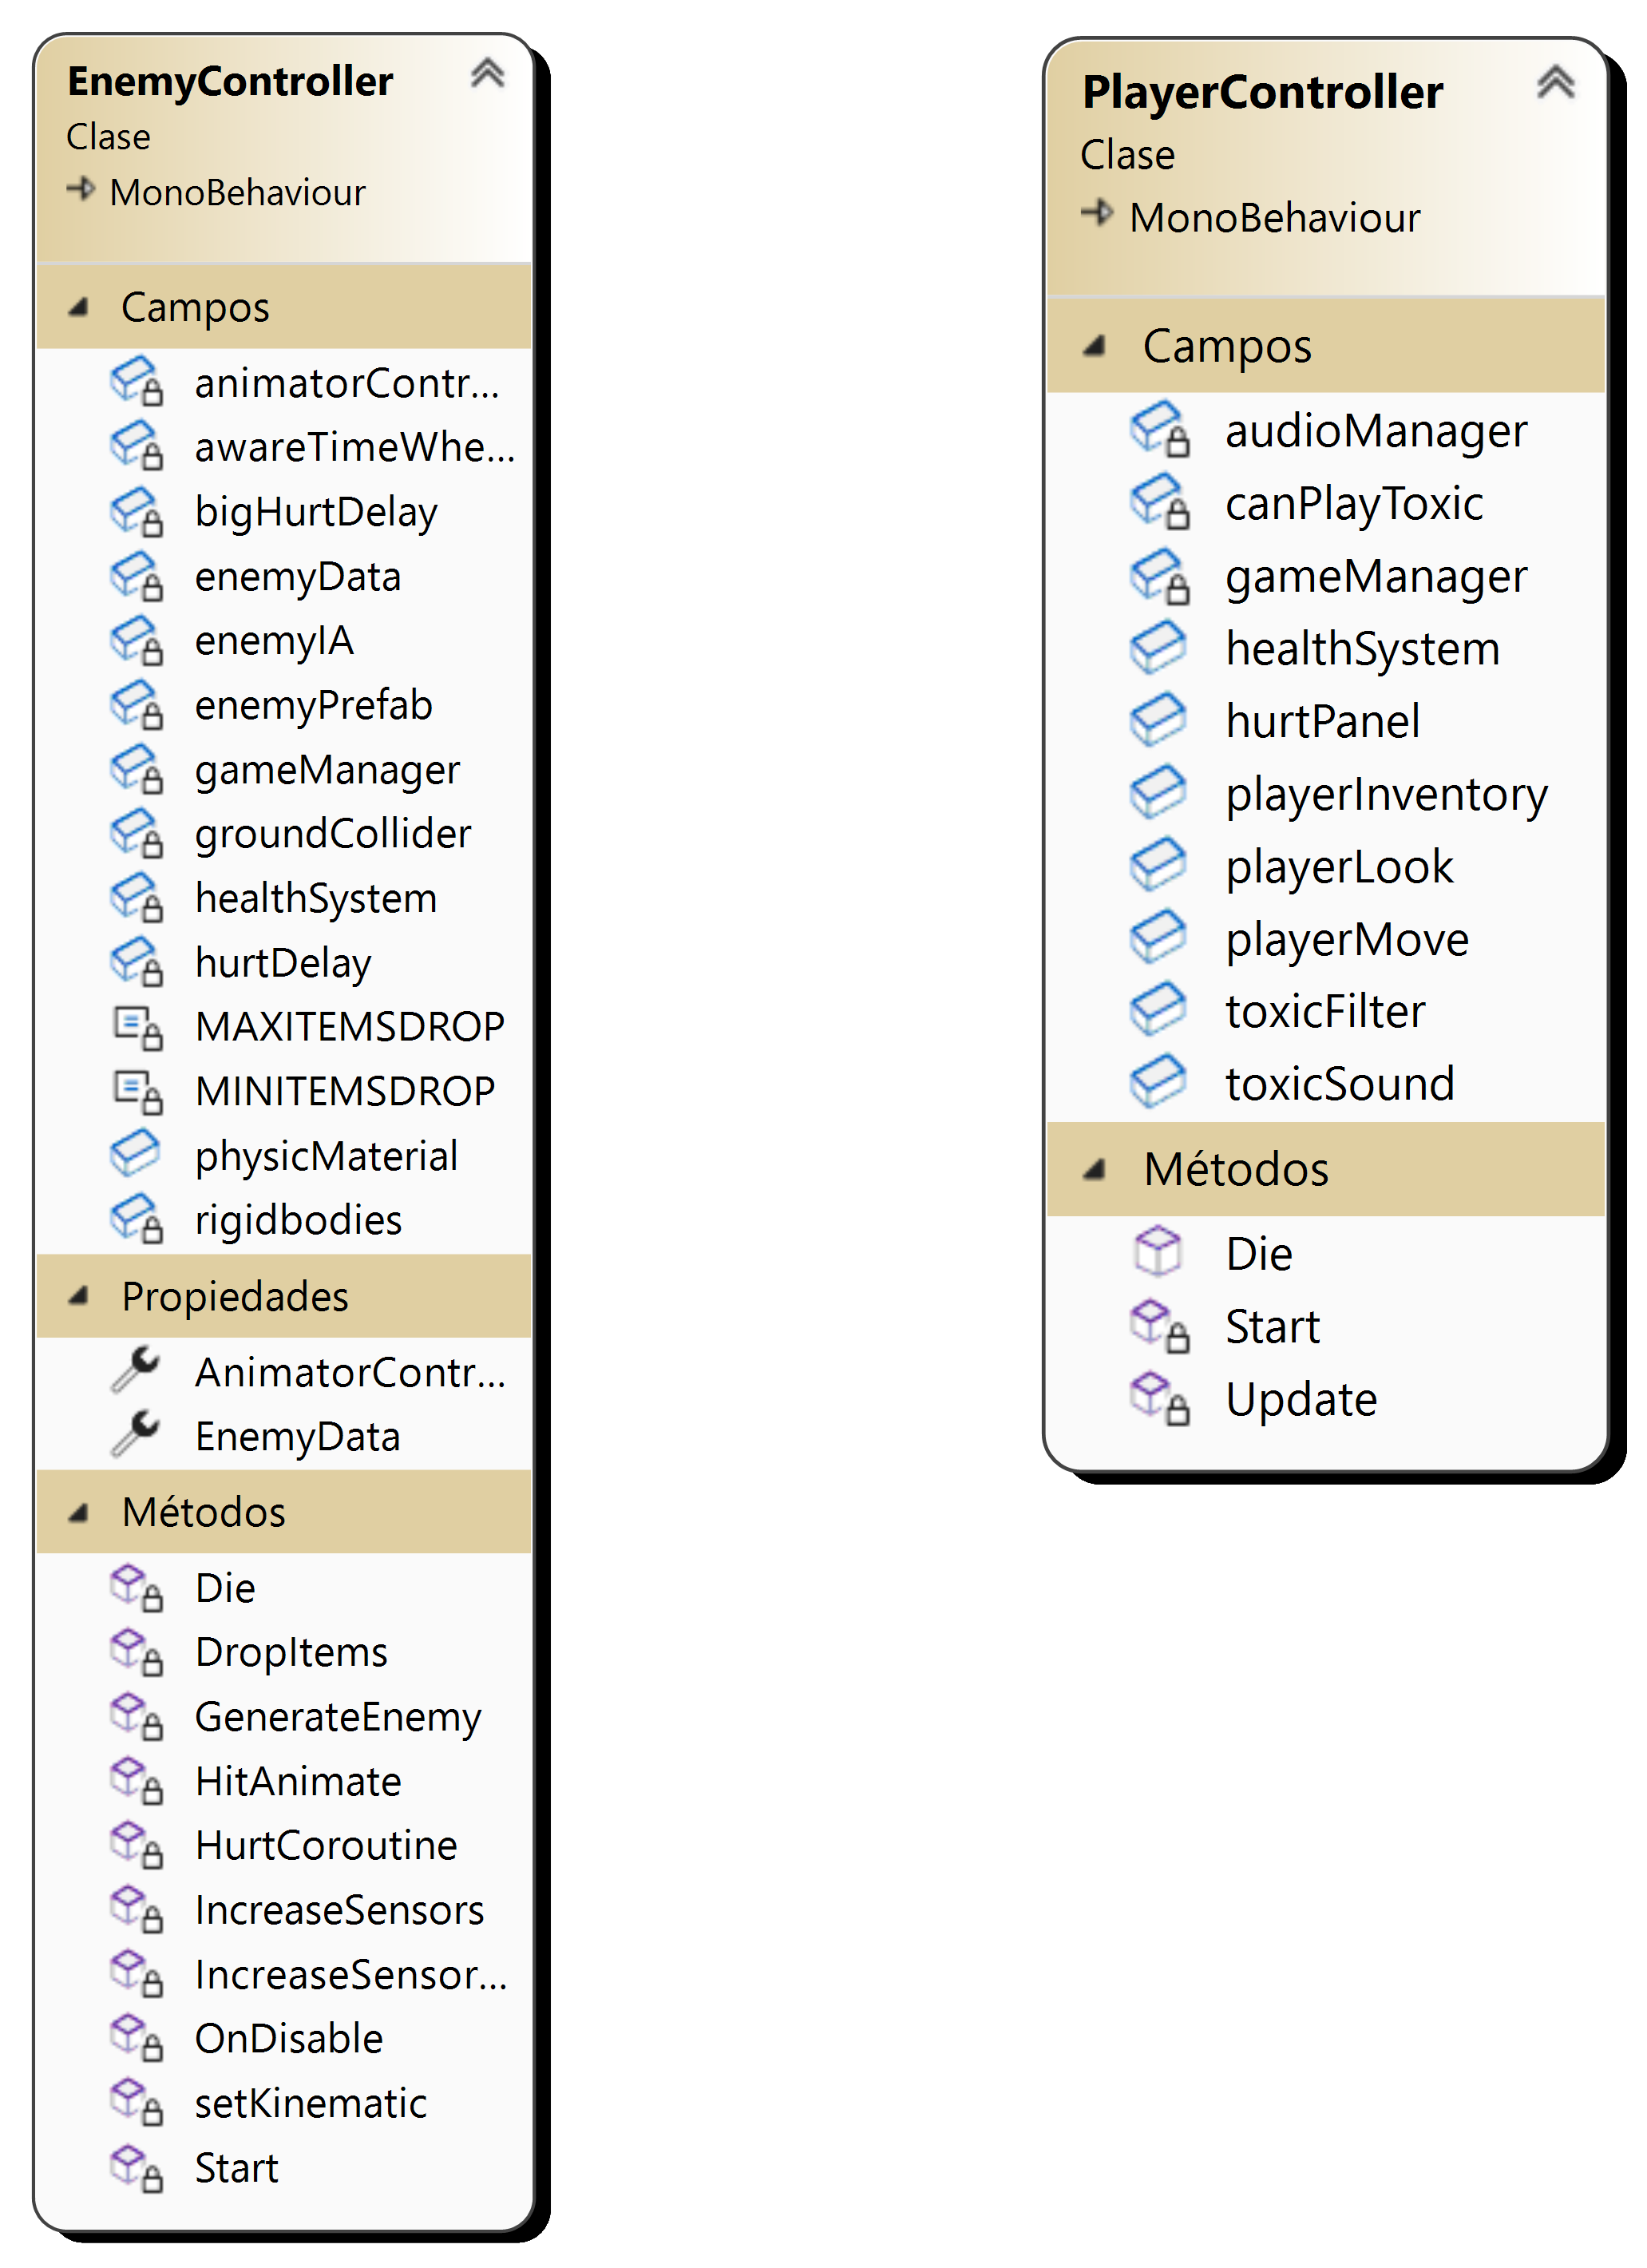
\includegraphics[scale=0.45]{img/PlayerAndEnemyControllers.png}
	\caption{Clases controladoras del jugador y los enemigos}
	\label{fig:ControladoresJugadorYEnemigo}
    \end{figure}
\textit{EnemyController}, por ejemplo, asigna los atributos y valores que tendrá el enemigo cuando se genere en la escena, monitoriza aspectos como la vida, la inteligencia, las animaciones, la interacción con el entorno, las colisiones, y gestiona sus diferentes componentes, desactivándolos cuando este muere, entre otros aspectos.

\subsection{ScriptableObjects}
Un aspecto muy relevante en el diseño de los datos del sistema ha sido el uso de los llamados ScriptableObjects. 

Los \textbf{\textit{ScriptableObjects}} son contenedores de datos con la peculiaridad de que son independientes de las instancias de clase, es decir, que a diferencia de las clases que heredan de \textit{MonoBehaviour}, los scriptableObjects no se pueden asociar a un GameObject como un componente más, sino que se guardan como un asset “estático” del proyecto, manteniéndose persistentes entre sesiones y accesibles mediante referencias.

Los datos almacenados en un scriptableObject son inmutables en el momento de ejecución, una vez la aplicación ha sido compilada, por lo que este tipo de contenedores son ideales para almacenar información que no cambiará durante la ejecución del programa y que vaya a ser consultada por varios objetos en la escena.

Por ejemplo, si se almacenan todos los datos de un gameobject en un script que herede de Monobehaviour y este se añade al gameobject como un componente, creando así un prefab, cada vez que se instancie dicho prefab, se cargará en memoria una copia completa de los datos por cada prefab que exista, lo que puede afectar gravemente al uso de memoria y, por tanto, al rendimiento de la aplicación.

Para solucionar esto, si hay datos del prefab que no son propios de cada instancia, sino comunes a todas ellas porque no van a cambiar durante la ejecución del programa, una mejor aproximación sería almacenar esta información como un scriptableObject, y después incluir en el script una referencia a este scriptableObject.

La razón de esto es que cuando en un script normal se referencia a un scriptableObject, solamente almacenan esa referencia que apunta al scriptableObject y no una copia completa de los datos que contiene. De esta forma se obtiene un mejor diseño de los datos, con un uso de memoria más optimizado y en general un mejor rendimiento de la aplicación.

En el proyecto se han utilizado 4 clases a modo de plantilla, que heredan de ScriptableObject para crear todos los scriptableObjects que se usan en el juego. Estas clases son \textbf{\textit{GranadeBlueprint}}, \textbf{\textit{WeaponBlueprint}}, \textbf{\textit{EnemyBlueprint}} e \textbf{\textit{ItemRarityBlueprint}} asociadas a los diferentes enemigos, granadas, rarezas de objetos y armas, respectivamente (ver figura \ref{fig:ScriptableObjects}).

\begin{figure}[h]
	\centering
	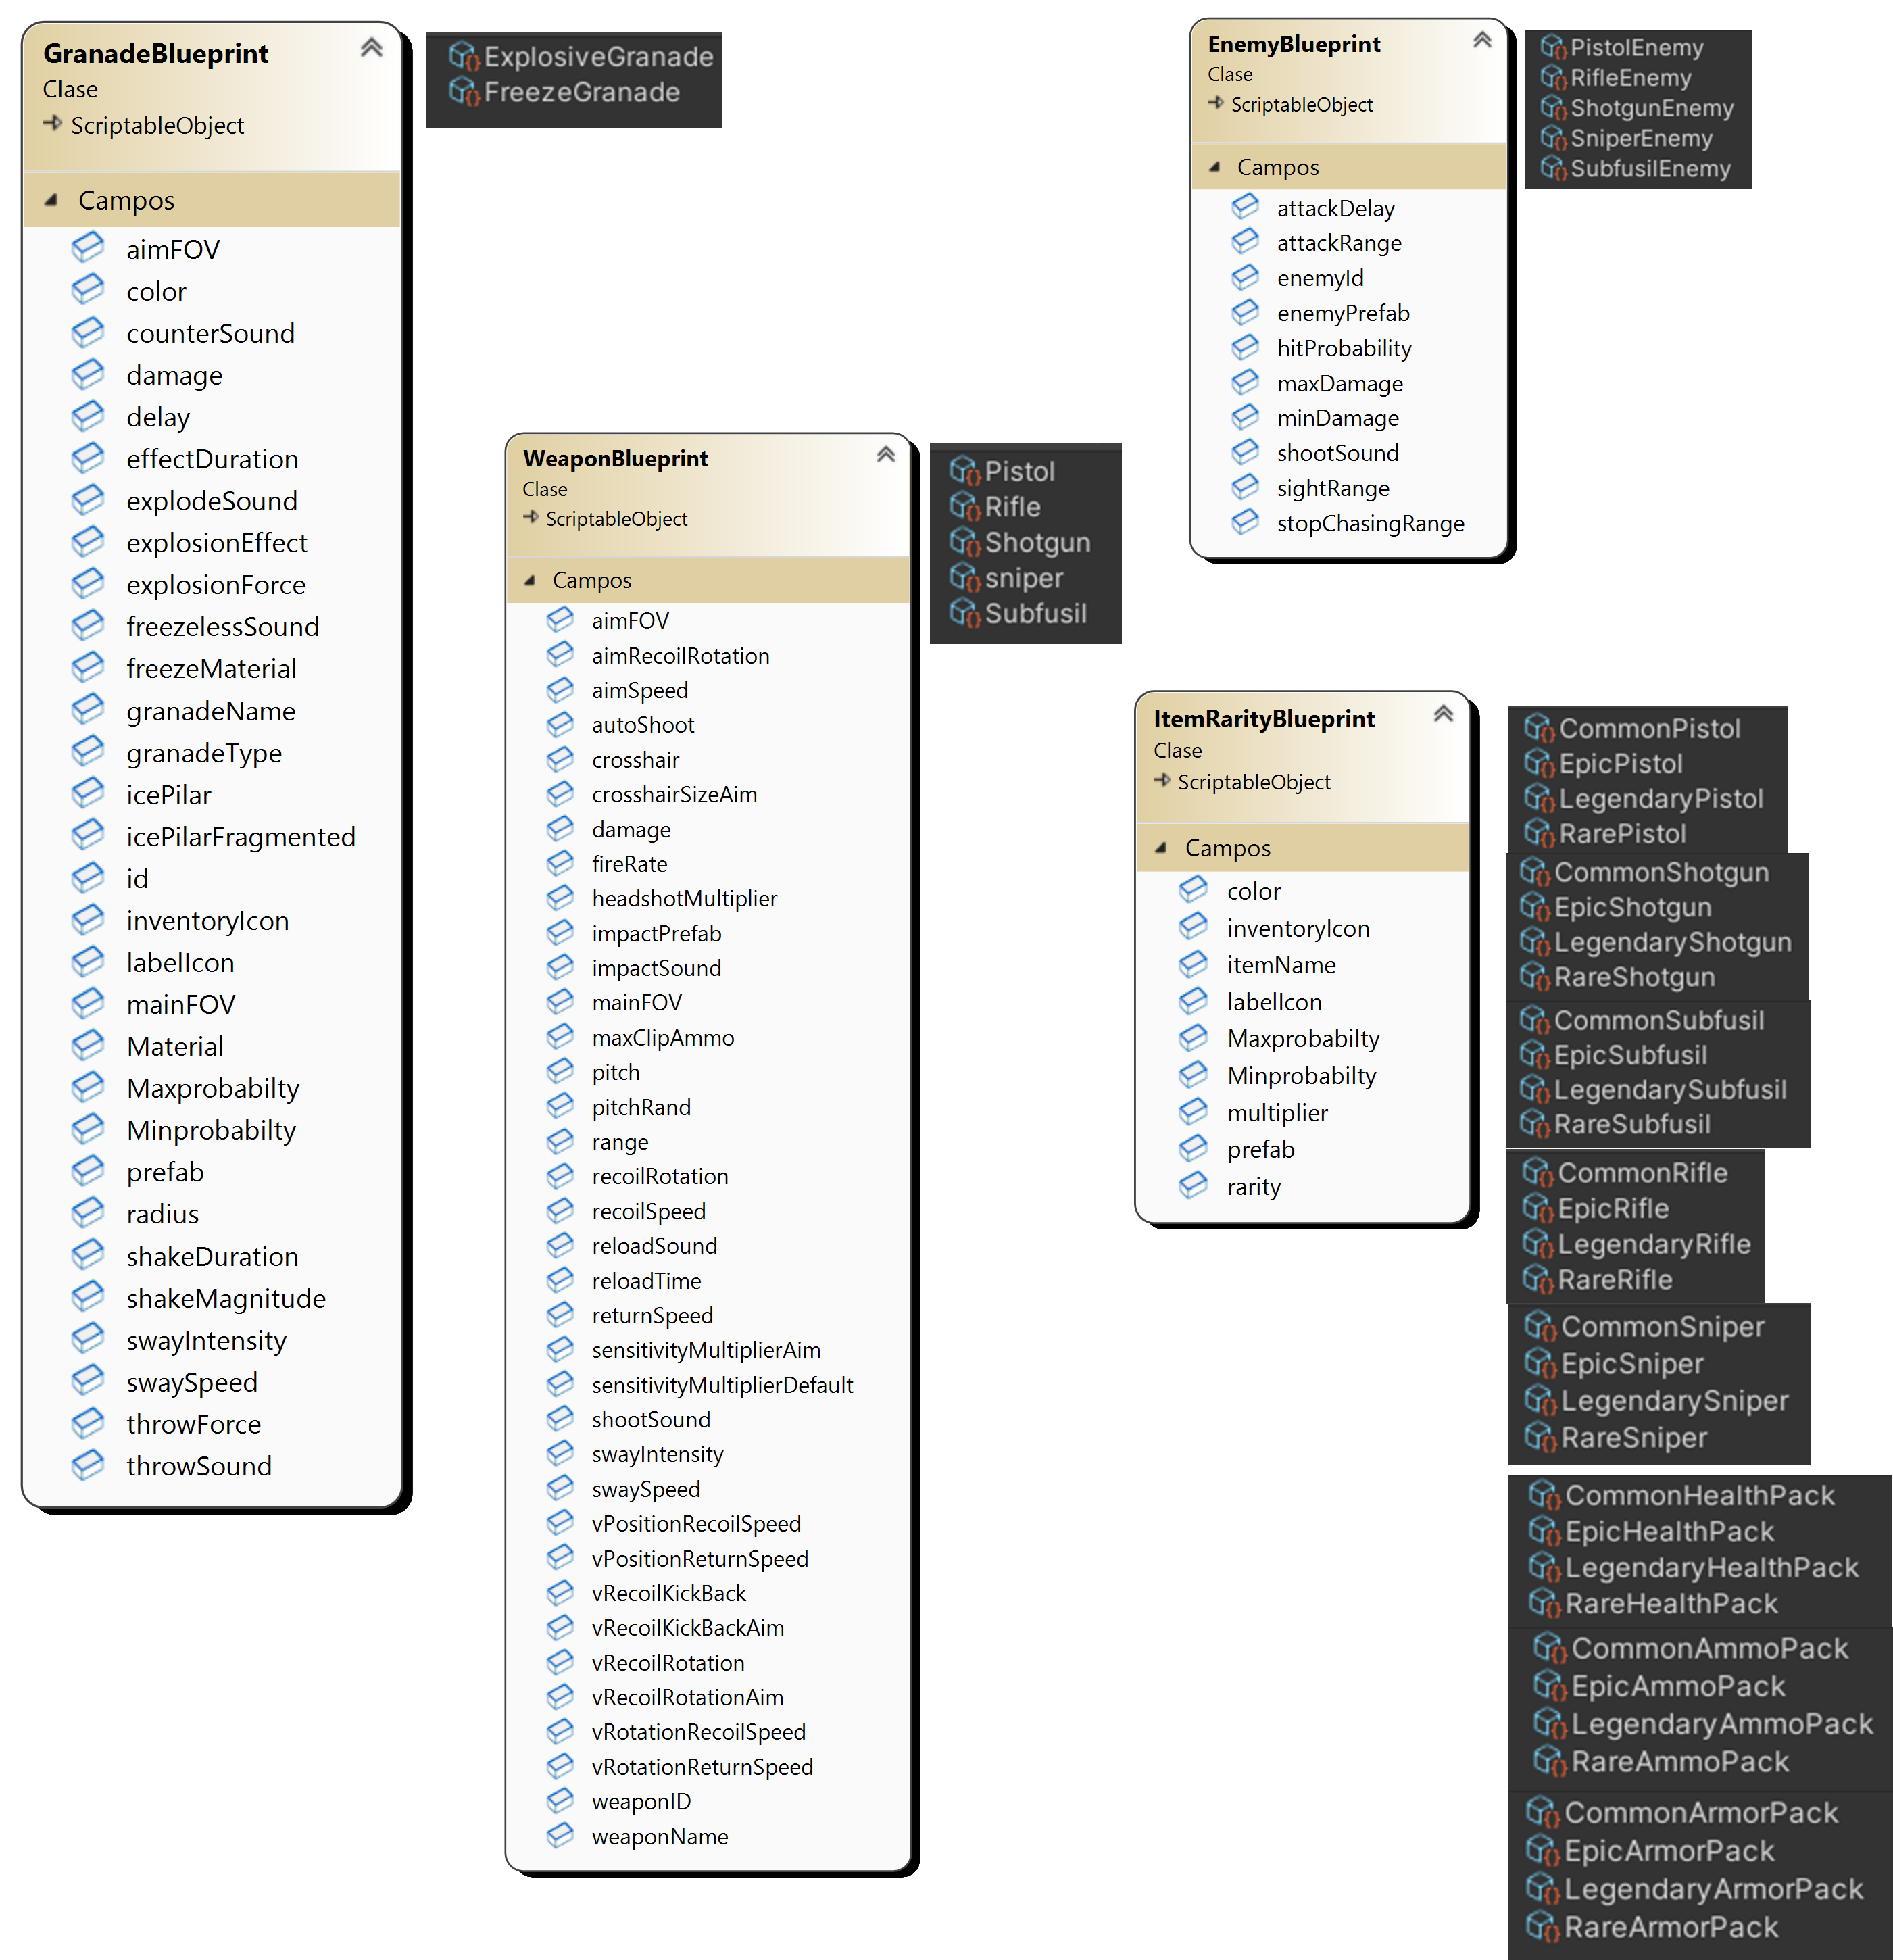
\includegraphics[scale=0.45]{img/Blueprints.png}
	\caption{Clases que heredan de ScriptableObject}
	\label{fig:ScriptableObjects}
    \end{figure}
    
Con el objetivo de ejemplificar el uso de estas estructuras de datos en el propio proyecto, se resumirá el flujo de trabajo con ScriptableObjects para la creación de los distintos tipos de enemigos que hay en el videojuego.

\subsubsection{Diseño de los enemigos}
Antes de crear un scriptableObject como tal se debe crear una clase que herede de la clase ScriptableObject, la cual actuará a modo de plantilla, con los datos que se desean almacenar. A partir de esta se crearán los diferentes scriptableObjects, cada uno con sus valores propios, que podrán ser usados más tarde en otros scripts.

La clase que actúa como plantilla de datos para los enemigos es \textit{EnemyBlueprint}, que, como se ha mencionado, deriva de la clase \textit{ScriptableObject}.

En este contenedor se deben definir los datos que se van a almacenar que, como se ha mencionado previamente, deben ser característicos del objeto (en este caso del enemigo) al que hagan referencia y no pueden cambiar una vez se inicie la aplicación.

Los datos que se mantendrán invariables, en este caso, son aspectos como el modelo 3D, el mínimo y máximo daño que puede hacer, el tiempo que hay entre sus ataques, la probabilidad de que acierte a su objetivo cuando dispare o su rango de vista y ataque. 

Sin embargo, otros atributos que sí irán cambiando a lo largo de la partida, como sus puntos de vida o su estado, deben almacenarse fuera de este contenedor para poder modificarse en tiempo de ejecución.

Una vez definidos los datos, se crean, a partir de esta plantilla, 5 assets desde el editor, todos con los mismos campos, que deben rellenarse con distintos valores en función de los tipos de enemigo que se quieran generar y sus características (ver figura \ref{fig:ScriptableObjectEnemigo}).
\begin{figure}[h]
	\centering
	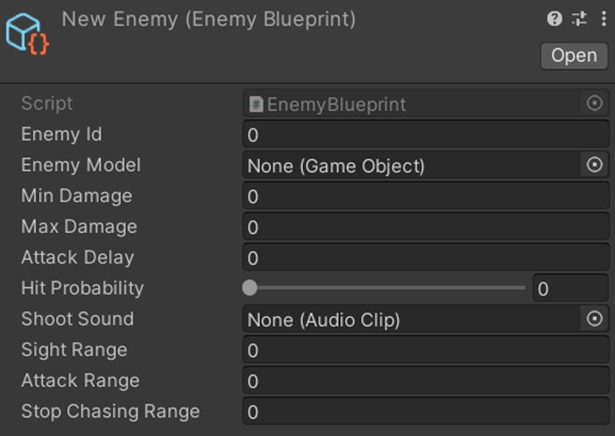
\includegraphics[scale=0.45]{img/EnemyScriptableObject.jpg}
	\caption{ScriptableObject de los enemigos}
	\label{fig:ScriptableObjectEnemigo}
    \end{figure}
Tras almacenar todos los valores estáticos de los posibles enemigos en diferentes scriptableObjects, se crea la ya mencionada clase \textit{EnemyController}, esta vez como típicamente se crea un script en el juego, heredando de \textit{MonoBehaviour}, en la que se incluye una referencia del tipo \textit{EnemyBlueprint}. Este atributo podrá referenciar a uno de los scriptableObjects del proyecto, al igual que el tipo int puede tomar los valores 1, 24 o 829.

De esta forma, se podrían crear \textbf{5 prefabs diferentes}, uno por cada tipo de enemigo en el juego y que cada uno contuviese una referencia al scriptableobject correspondiente.

En este caso, no se conocerá de antemano el tipo de enemigo que va a representar un prefab \textit{enemy} al momento de arrastrarlo a la escena, sino que será el \textit{GameManager} (es allí donde se tiene un array de referencias a todos los scriptableobjects) quien escoja aleatoriamente un scriptableObject de un tipo de enemigo, y después el \textit{EnemyController} ligado al prefab, construirá el enemigo escogido con los datos del scriptableobject elegido.   

Utilizando este diseño en los datos, se consigue tener un único prefab para generar todos los enemigos del juego (ver figura \ref{fig:PrefabEnemigos}).
\begin{figure}[h]
	\centering
	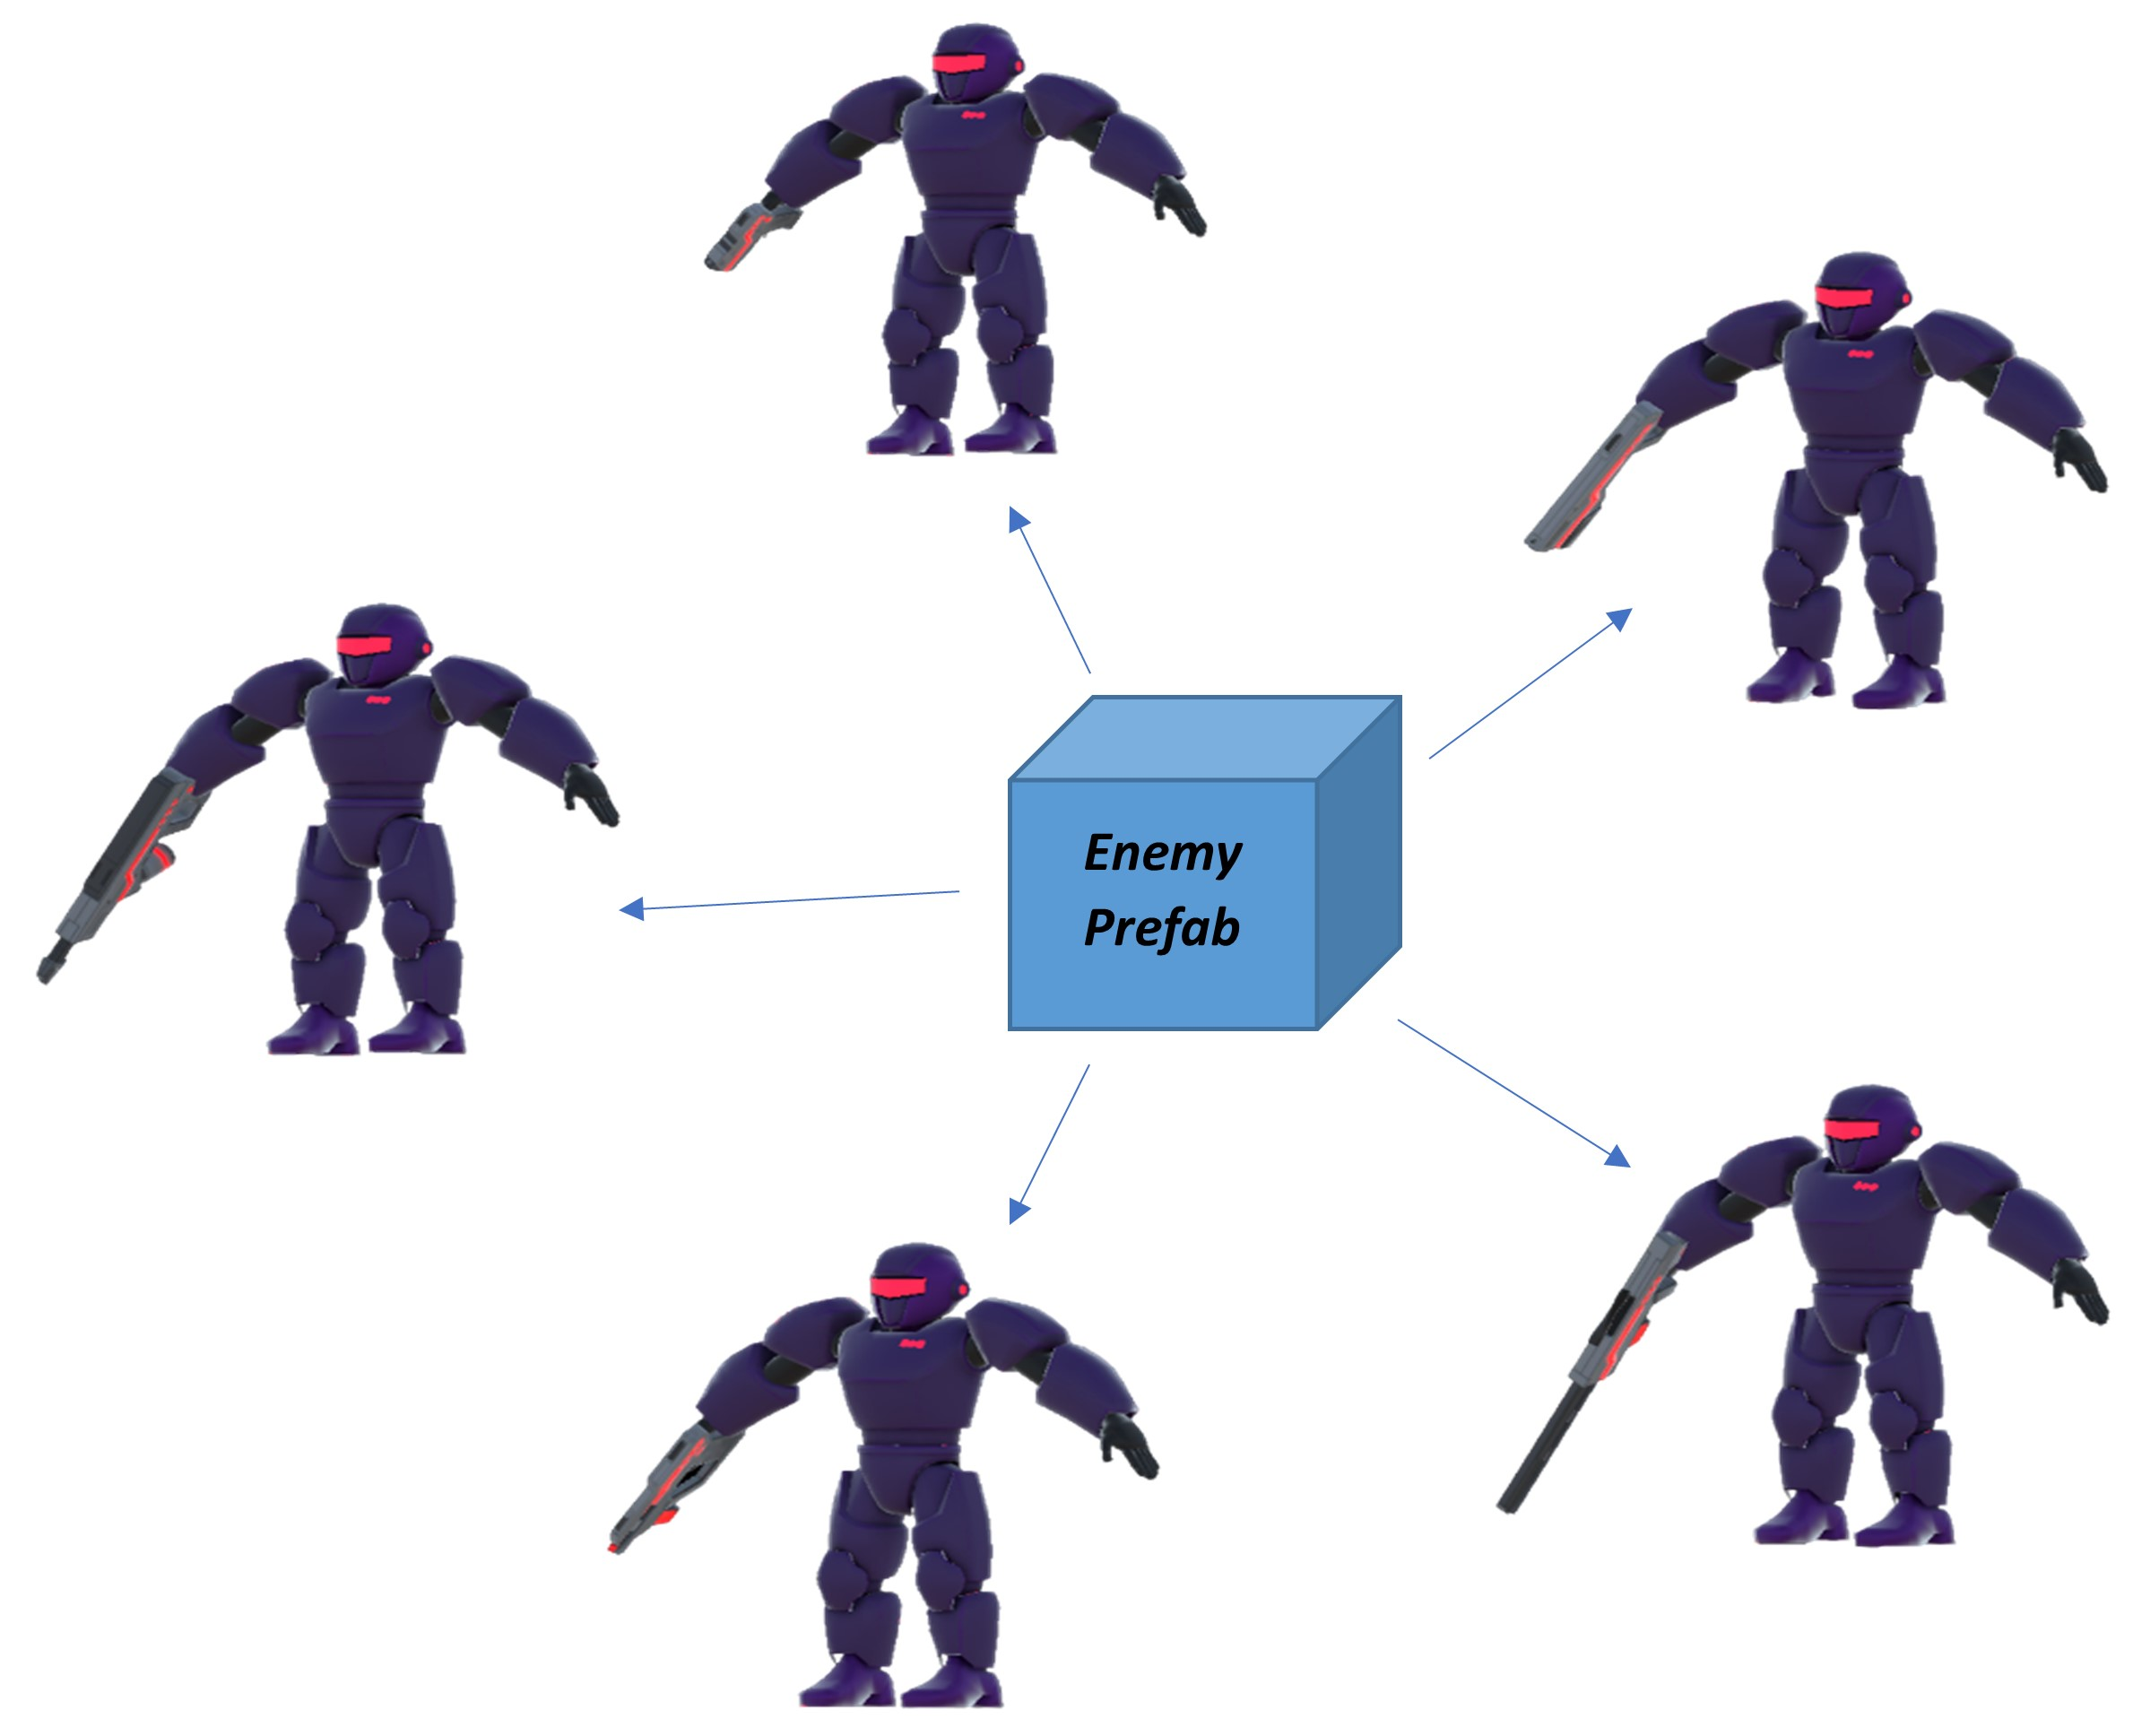
\includegraphics[scale=0.45]{img/EnemyPrefab.jpg}
	\caption{Único prefab para todos los enemigos}
	\label{fig:PrefabEnemigos}
    \end{figure}
Además, gracias a los scriptableObjects, cada vez que se instancie un enemigo de un tipo, los datos comunes a ese tipo no se duplicarán sino que accederán todos al mismo contenedor de datos (ver figura \ref{fig:PistolEnemyScriptableObject}), algo que mejora en gran medida la eficiencia general del programa y más, teniendo en cuenta la gran cantidad de enemigos que puede haber simultáneamente en este género de videojuegos (50-100).
\begin{figure}[h]
	\centering
	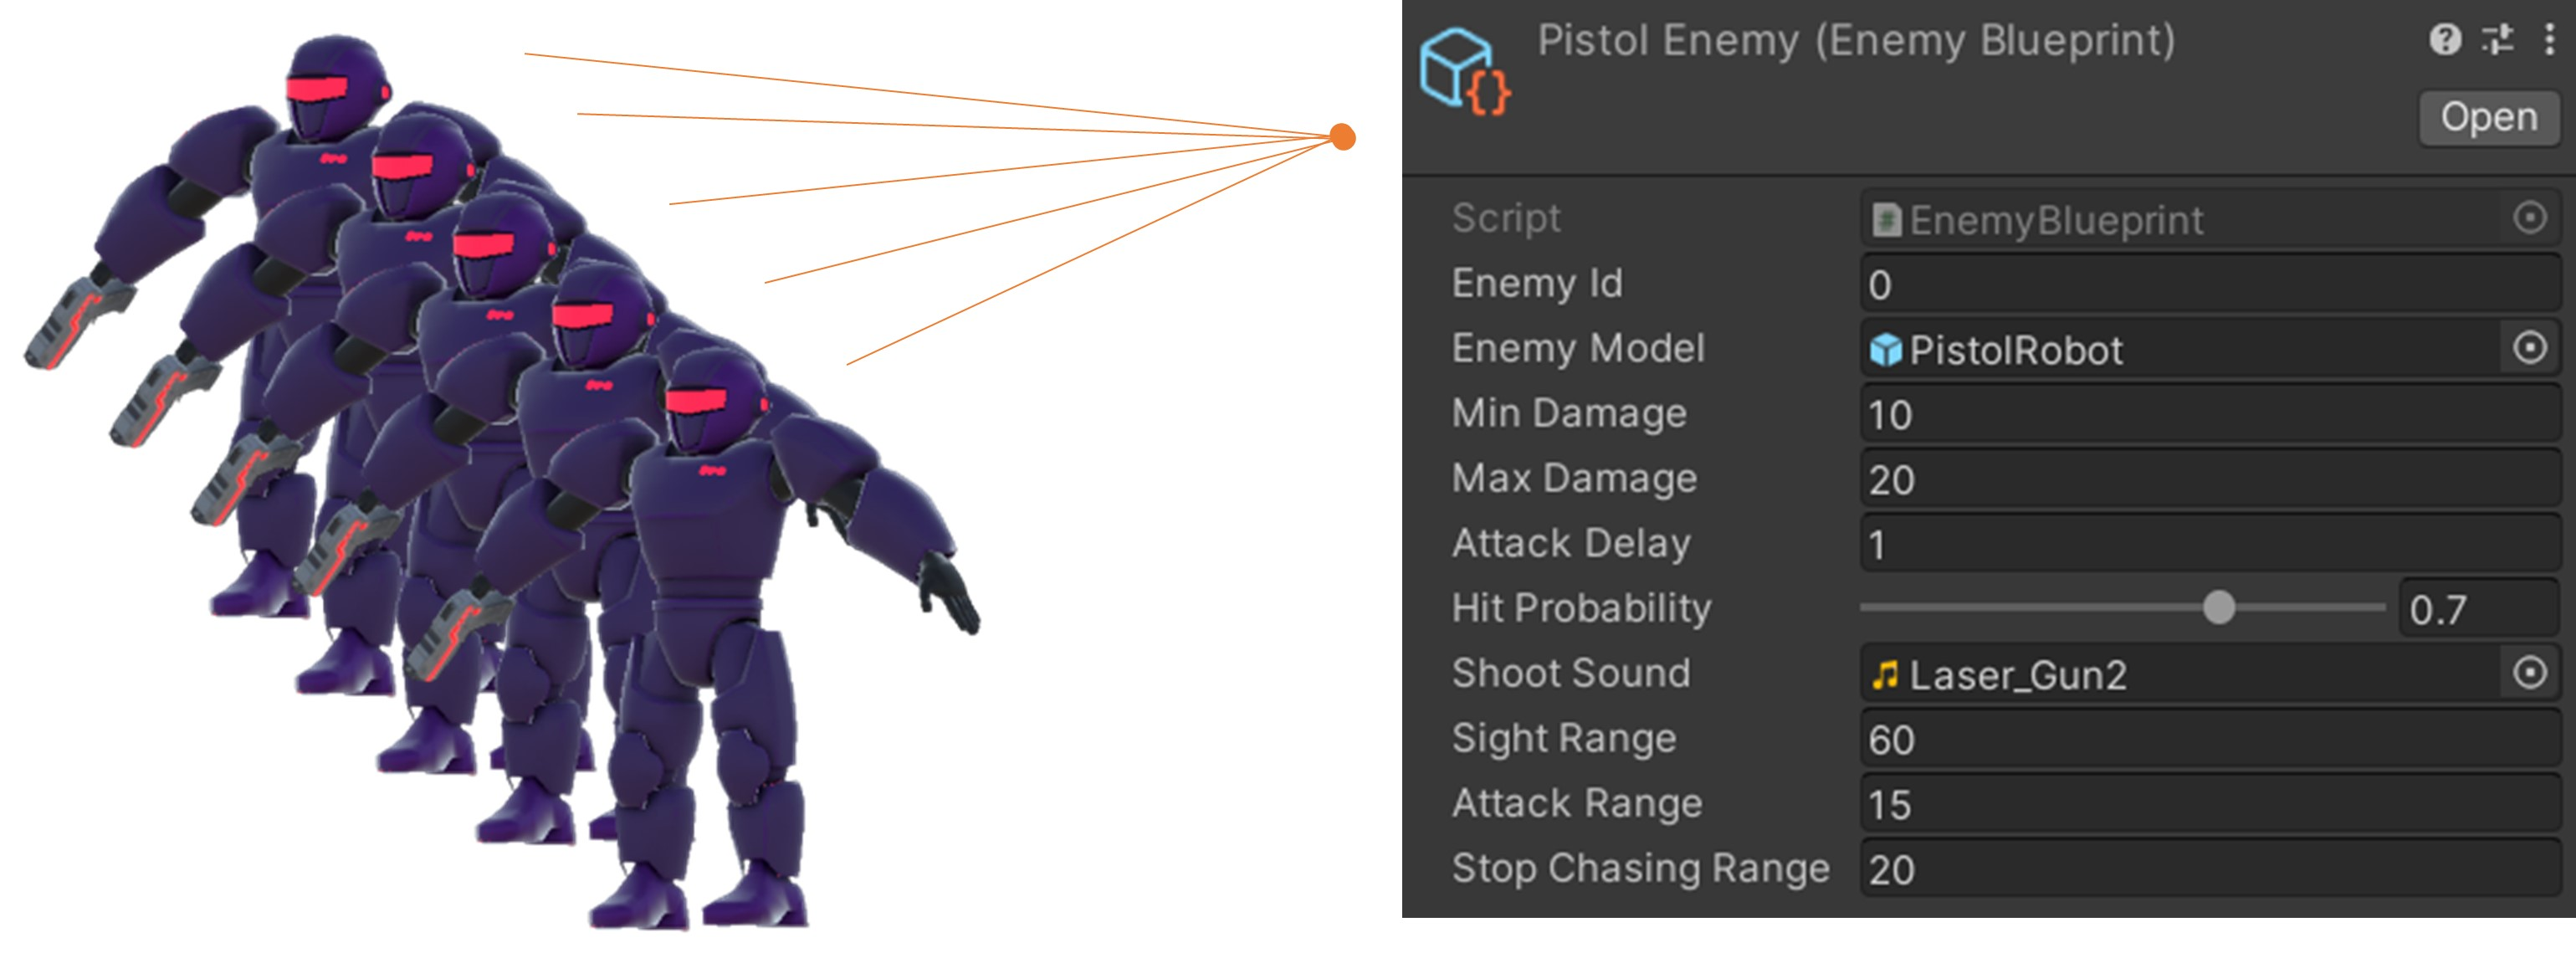
\includegraphics[scale=0.45]{img/PistolEnemyScriptableObject.jpg}
	\caption{Varios objetos acceden al mismo contenedor de datos}
	\label{fig:PistolEnemyScriptableObject}
    \end{figure}
Es más, atendiendo al objetivo de escalabilidad y \textbf{extensibilidad}, si se desea añadir un nuevo tipo de enemigo al juego, simplemente se tendría que crear un nuevo scriptableObject a partir de la plantilla, rellenar sus campos y añadir ese objeto al array de referencias de enemigos en la clase GameManager, facilitando así el proceso de incluir nuevo contenido al videojuego.

De esta forma, al arrastrar el Prefab del enemigo a la escena, el nuevo tipo de enemigo ya sería candidato para generarse por el Prefab cuando se inicie el programa.

En los diagramas de clases mostrados en este apartado se puede observar que no hay clases que hereden unas de otras, y es que los scriptableobjects sustituyen en gran medida a clases genéricas, ya que son contenedores con atributos comunes, que bien podrían representar este tipo de clases si no existiesen los scriptableObjects.

\subsection{Events} \label{Events}
Otro elemento clave en el diseño de los datos de la aplicación para que la información de las clases se comunique entre sí son los llamados eventos (\textit{events}) de Unity.

Un \textbf{\textit{event}} no es más que una forma de anunciar que algo concreto ha pasado en algún script, para quien quiera escucharlo, lo sepa.

En un evento hay dos tipos de participantes. Quien envía el evento se llama \textbf{\textit{publisher}}, y quienes lo escuchan se denominan \textbf{\textit{subscribers}} o suscriptores. Cuando algo concreto ocurre, el \textit{Publisher} anuncia el evento, y los subscribers son notificados de que el evento ha ocurrido.

La clave de este diseño es que el \textit{Publisher} no sabe quiénes son sus suscriptores, si los tuviera, lo que permite obtener modularidad en el traspaso de datos, teniendo, por un lado, el código principal en el Publisher y, por otro lado, en los subscribers, funcionalidades adicionales no esenciales a la acción del Publisher.

En el videojuego se han utilizado los eventos principalmente para mantener la \textbf{lógica separada de lo visual} en elementos como el inventario o el sistema de salud. De esta manera, la lógica puede seguir funcionando aún sin los elementos visuales, ya que no contendrá ningún tipo de referencia hacia ellos.\\
También permite reutilizar más fácilmente el código del Publisher y añadir nuevos elementos visuales asociados a él más fácilmente, lo que responde a los objetivos de usabilidad, extensibilidad y eficiencia.

A continuación se describe el diseño del sistema de salud y cómo utiliza los \textit{events}.

La clase \textbf{\textit{HealthSystem}} contiene toda la lógica del sistema de salud tanto del jugador como de los enemigos. Será por tanto quien publique los eventos. Se definen 4 eventos diferentes (ver figura \ref{fig:EventosHealthSystem}), asociados a los principales sucesos que pueden ocurrir en en esta clase: Recibir daño, recuperar salud, recuperar armadura, y morir.

\begin{figure}[h]
	\centering
	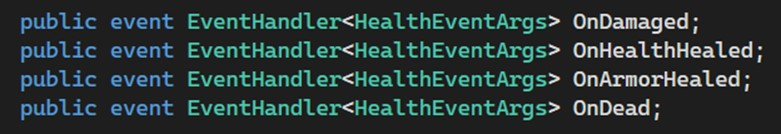
\includegraphics[scale=0.45]{img/HealthEventArgs.jpg}
	\caption{Definición de eventos en la clase ``HealthSystem''}
	\label{fig:EventosHealthSystem}
    \end{figure}
    
Cabe destacar que cuando se anuncia un evento, este puede contener algunos \textbf{argumentos} que se enviarán junto al evento para que los subscribers puedan trabajar con ellos. El tipo de argumentos que se pueden usar se debe definir en clases especiales que hereden de la clase \textit{EventArgs}.

En este ejemplo, los eventos de la clase \textit{HealthSystem} podrán utilizar los argumentos definidos en la clase \textbf{\textit{HealthEventArgs}}.

De esta manera, cuando, por ejemplo, se llame al método \textbf{\textit{HealHealth(int amount)}} de la clase, además de la lógica pertinente que realice el método, como sumar \textit{amount} puntos de vida al atributo referente a la salud, \textbf{se disparará el evento \textit{OnHealthHealed}}, con \textit{amount} como argumento, anunciando que se ha recuperado cierta cantidad de salud en dicha instancia de la clase.\\
Las clases que estén suscritas a dicho evento serán notificadas y realizarán alguna acción al respecto.

La clase \textit{HealthSystemVisuals} es la encargada de actualizar todos los elementos visuales relacionados con la salud, como las barras de salud y armadura, los puntos de vida del jugador, los textos flotantes que aparecen al hacer daño a un enemigo o los efectos visuales y sonoros de daño, cura y armadura, entre otros.

Con el fin de poder actualizar dichos elementos, la clase está suscrita a los eventos que publica la clase \textit{HealthSystemVisuals} para así poder estar al tanto de sucesos que le interesan .

Para suscribirse a un evento y poder realizar una acción asociada a él se utiliza esta sencilla nomenclatura: \textbf{Evento += acción a realizar} (ver figura \ref{fig:SuscripcionesHealth}). De manera similar, si se desea que una clase deje de prestar atención a un evento, se utiliza la nomenclatura \textbf{Evento -= acción a realizar}.

\begin{figure}[h]
	\centering
	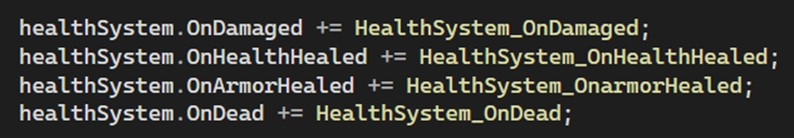
\includegraphics[scale=0.45]{img/HealthSystemVisuals.jpg}
	\caption{Suscripciones en la clase ``HealthSystemVisuals''}
	\label{fig:SuscripcionesHealth}
    \end{figure}
    
De esta manera, a modo de resumen, cuando se dispare el evento \textit{OnHealthHealed} en la instancia de \textit{HealthSystem} del jugador, la instancia correspondiente de \textit{HealthSystemVisuals} llamará a su método \textit{HealthSystem\_OnHealthHealed} para realizar acciones asociadas al evento, como actualizar la barra de salud del jugador y sus puntos de vida en la interfaz o reproducir el sonido y los efectos visuales asociados a la curación (ver figura \ref{fig:UMLHealth}).

\begin{figure}[h]
	\centering
	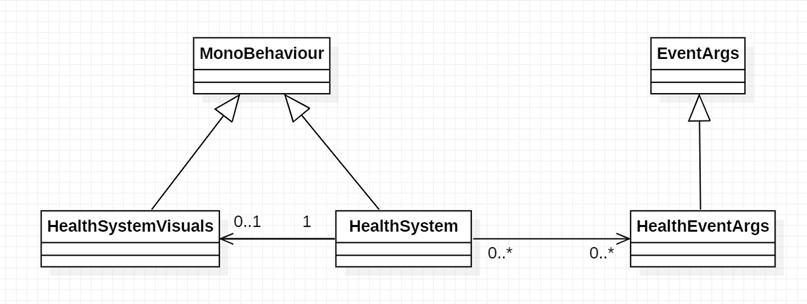
\includegraphics[scale=0.45]{img/UMLClassDiagram.jpg}
	\caption{Diagrama de clases UML del sistema de salud}
	\label{fig:UMLHealth}
    \end{figure}
    
Este método para separar los datos lógicos de los visuales se utiliza de manera similar en la clase \textbf{\textit{PlayerInventory}} (ver figuras \ref{fig:EventosInventario} y \ref{fig:SuscripcionesInventario}), que gestiona la parte lógica del inventario del jugador. En este caso, los eventos serán propios de un inventario, como añadir un objeto, tirar un objeto o cambiar el objeto activo, y la clase que escuche dichos eventos será \textbf{\textit{InventoryVisuals}}.

\begin{figure}[h]
	\centering
	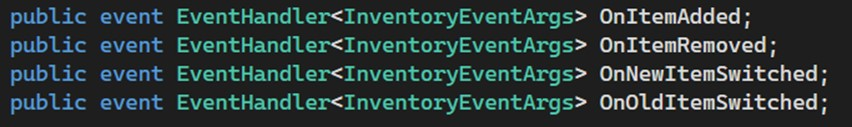
\includegraphics[scale=0.45]{img/InventoryEvents.jpg}
	\caption{Definición de eventos en la clase “PlayerInventory”}
	\label{fig:EventosInventario}
\end{figure}

\begin{figure}[h]
    \centering
    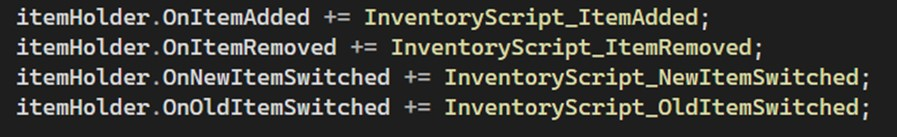
\includegraphics[scale=0.45]{img/InventorySubscribers.jpg}
    \caption{Suscripciones en la clase “InventoryVisuals”}
    \label{fig:SuscripcionesInventario}
\end{figure}
El uso de eventos en Unity es imprescindible para que los diferentes elementos se comuniquen entre sí de manera eficiente y se disponga de una estructura de clases adecuada con un código limpio y fácil de mantener (ver figura \ref{fig:EsquemaEventos}).

\begin{figure}[h]
    \centering
    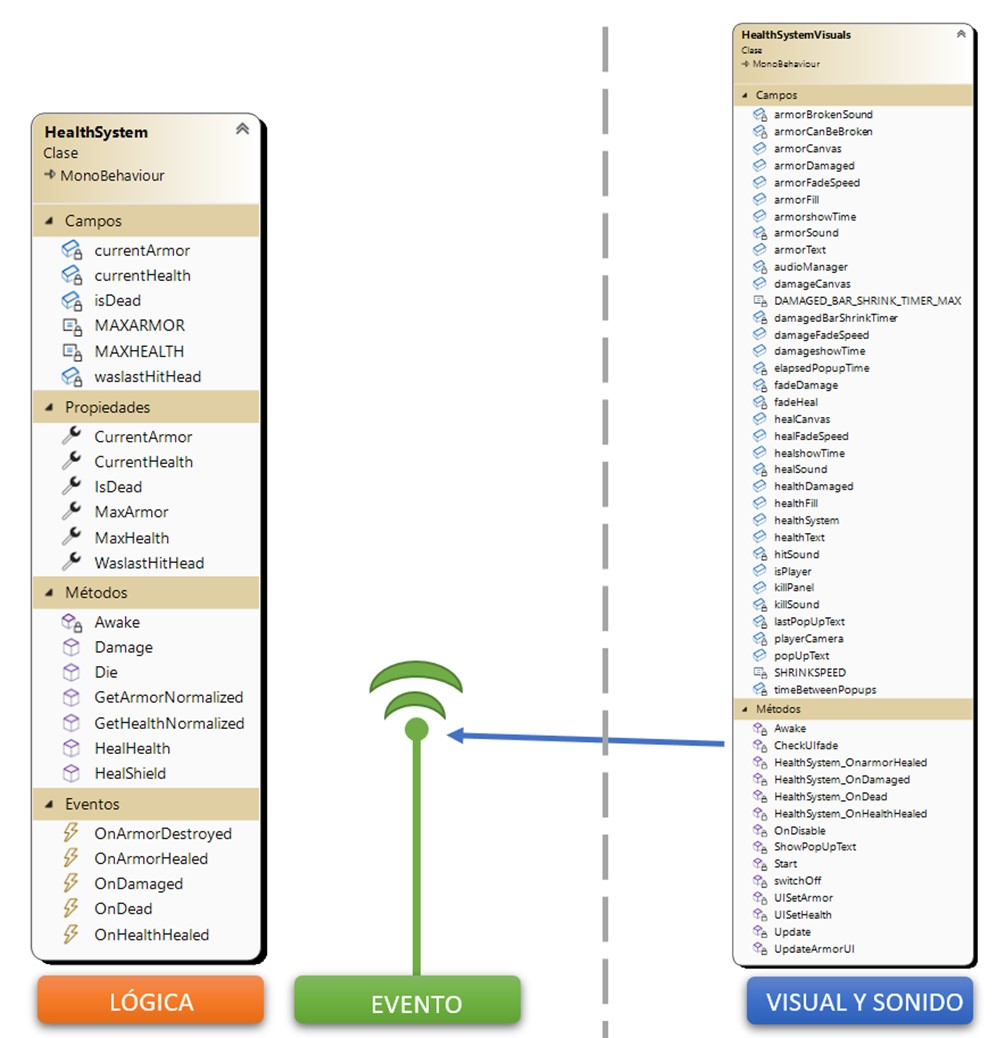
\includegraphics[scale=0.45]{img/EventsUnity.jpg}
    \caption{Esquema del funcionamiento de los eventos}
    \label{fig:EsquemaEventos}
\end{figure}

\subsection{Añadir arma nueva al juego}

Para ilustrar cómo se integran todos estos datos en el proyecto, se puede ver, por ejemplo, el proceso a través del cual se añade un nuevo tipo de arma al juego, ya que en él se incluyen varios de los elementos descritos anteriormente.

\begin{enumerate}
    \item \textbf{\textit{Crear recursos de diseño del arma}}
    Al querer incluir un arma nueva en el juego, se han de crear antes los elementos artísticos que van a componerla, como su modelo 3D, sus texturas o los efectos de sonido.
    
    Se ha utilizado el programa \textit{Audacity} \cite{wiki:Audacity} para crear y mezclar los sonidos de disparo y de recarga de todas las armas (ver figura \ref{fig:SonidosAudacity}).
    \begin{figure}[h]
    \centering
    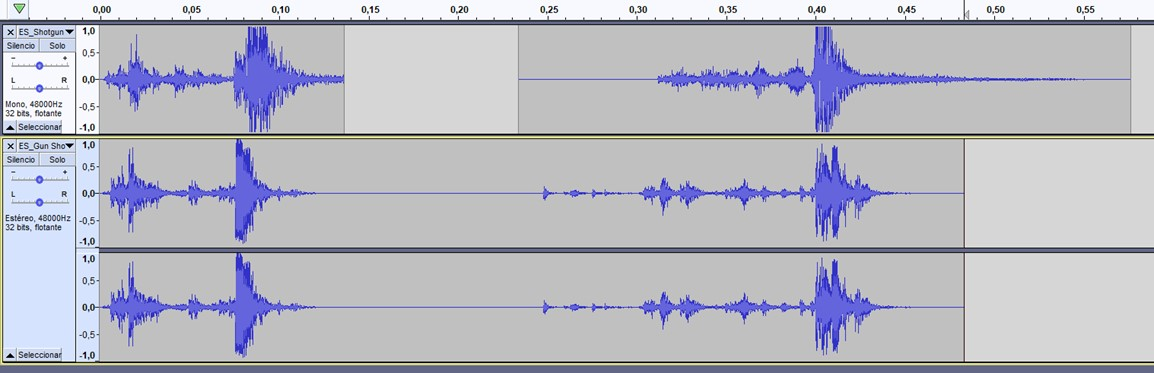
\includegraphics[scale=0.45]{img/AudacityScreenshot.jpg}
    \caption{Captura de Audacity con el sonido de Recarga de la escopeta}
    \label{fig:SonidosAudacity}
    \end{figure}
    Para los modelos 3D de las armas, se ha adquirido un pack de modelos en la tienda de Unity, en conjunción con el programa \textit{Blender} \cite{wiki:Blender} para crear partes nuevas o adaptar y modificar las existentes (por ejemplo para crear la mirilla telescópica del francotirador, que inicalmente no existía).\\
    En el caso concreto de la escopeta, se ha utilizado blender para crear y añadir la parte corredera de esta y diseñar su color y textura (ver figura \ref{fig:EscopetaBlender}).
    
    \begin{figure}[h]
    \centering
    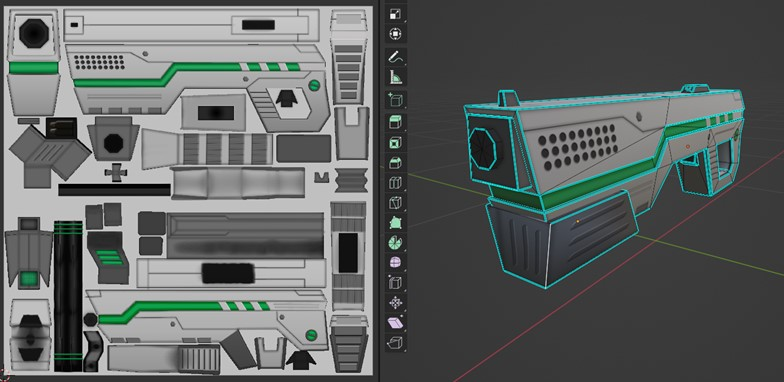
\includegraphics[scale=0.45]{img/ShotgunBlender.jpg}
    \caption{Modelo y textura princial de la escopeta}
    \label{fig:EscopetaBlender}
    \end{figure}
    
    \item \textbf{\textit{Importar los recursos a Unity}}
    Una vez se han creado los elementos necesarios, se deben importar a Unity en el formato adecuado para que se creen los assets correspondientes. Por ejemplo, los modelos de blender se pueden importan en formato .blend o .fbx, mientras que las pistas de audio se importan en formato .wav para que sean compatibles con el motor.
    Las texturas se suelen importar en formato .png.
    
    \item \textbf{\textit{Construir modelo y materiales}}
    Ya en Unity, se crea el material del arma con las texturas adecuadas y se añaden los atributos necesarios, como correcciones del color o diferentes mapas. Los mapas utilizados en el material del arma son la textura base, un mapa de normales o \textit{normal map}, que crea relieve de manera artificial en la textura, y un mapa de emisión o \textit{emission map}, que delimita las zonas de la textura que deben emitir luz. En este caso, la zona que debe brillar es la del color neón del arma (ver figura \ref{fig:TexturasEscopeta}).
    
    \begin{figure}[h]
    \centering
    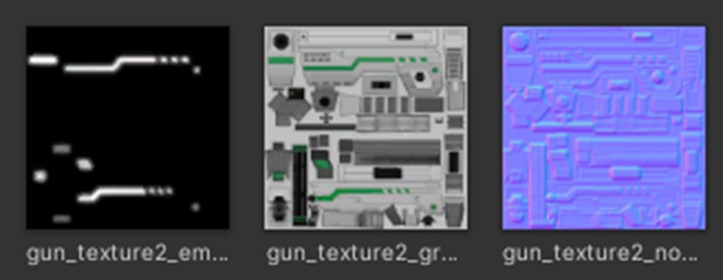
\includegraphics[scale=0.45]{img/ShotgunTexture.jpg}
    \caption{Mapas de texturas de la escopeta}
    \label{fig:TexturasEscopeta}
    \end{figure}
    
    Una vez creado el material, se adhiere al arma y después se acopla el arma al modelo de brazos del jugador para tener así el modelo completo que se verá una vez se sostenga el arma en primera persona (ver figura \ref{fig:Escopeta}).
    \\No hace falta crear un modelo nuevo por cada rareza que tenga el arma; basta con duplicar el modelo y asignar los diferentes materiales asociados a cada una de las rarezas para poder diferenciar los modelos.
    
    \begin{figure}[h]
    \centering
    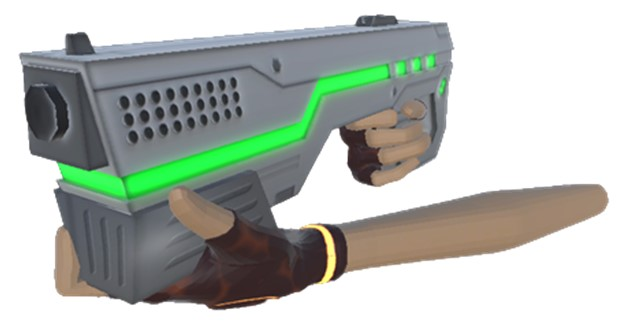
\includegraphics[scale=0.45]{img/Shotgun.jpg}
    \caption{Modelo completo de la escopeta en Unity}
    \label{fig:Escopeta}
    \end{figure}
    
    \item \textbf{\textit{Crear las animaciones del arma}}
    En este paso se deben crear todas las animaciones necesarias para el arma importada. También se pueden hacer en blender, como se ha hecho con otros objetos como las cajas de suministro, pero en este caso se ha preferido hacer directamente en Unity por conveniencia.\\
    En el caso de la escopeta, al igual que para el resto de armas, las animaciones necesarias son la que se ve al sacar el arma para utilizarla y la de recargar (ver figura \ref{fig:AnimacionEscopeta}), además de una adicional para cuando el arma esté en estado nuetro (sin hacer ninguna acción).
    
    Cabe mencionar que la acción de disparar se anima de forma procedural por código, por lo que no es necesario crear una animación específica de disparo (esto se explica más a fondo en la sección \textit{Aspectos relevantes del proyecto} de la memoria.
    \begin{figure}[h]
    \centering
    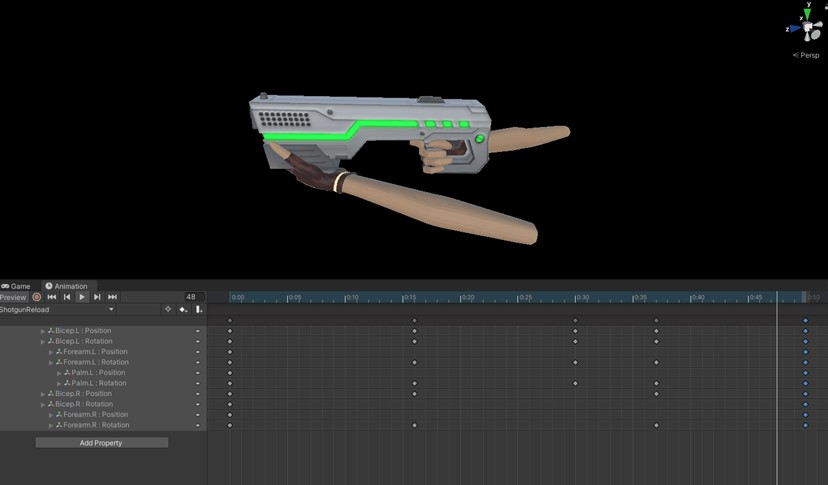
\includegraphics[scale=0.45]{img/ReloadingShotgun.jpg}
    \caption{Proceso de animación de recarga para la escopeta}
    \label{fig:AnimacionEscopeta}
    \end{figure}
    Una vez creadas todas las animaciones, se configura un nuevo \textbf{\textit{Animator Controller}}, que se encargará de supervisar el flujo y la transición de las animaciones en el orden y momento adecuados a través de una \textbf{\textit{State Machine}} o Máquina de estados (ver figuras \ref{fig:AnimatorEscopeta} y \ref{fig:EstadosEscopeta}).
    
    Por ejemplo, cuando el jugador tenga equipada el arma, no tenga el cargador lleno y pulse la tecla ``R'', se reproducirá la animación de recarga para que el jugador obtenga un feedback visual de la acción.
    
    \begin{figure}[h]
    \centering
    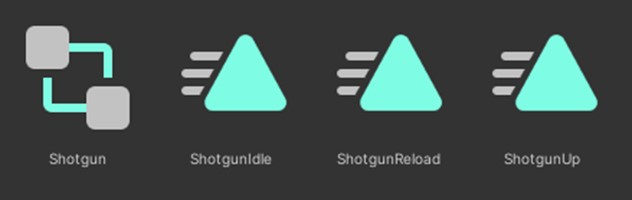
\includegraphics[scale=0.45]{img/ShotgunAnimatorController.jpg}
    \caption{Animator y animaciones de la escopeta}
    \label{fig:AnimatorEscopeta}
    \end{figure}
    
    \begin{figure}[h]
    \centering
    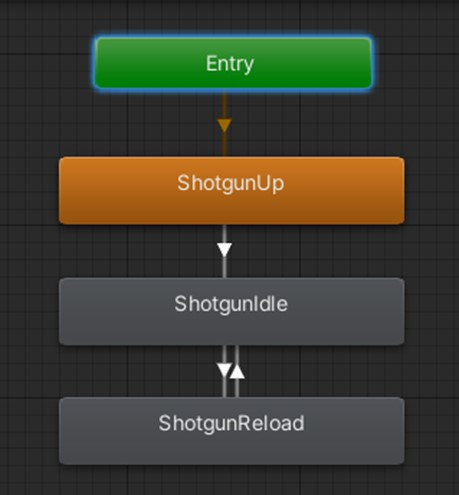
\includegraphics[scale=0.45]{img/StateMachine.jpg}
    \caption{Máquina de estados de las animaciones de la escopeta}
    \label{fig:EstadosEscopeta}
    \end{figure}
    
    \item \textbf{\textit{Crear scriptableObject del arma}}
    Ahora que ya se tienen listos todos los recursos visuales y sonoros del arma, se empieza a generar la lógica de esta. Para seguir con el flujo de datos diseñado para la lógica de las armas, se debe crear un scriptableobjet asociado a la escopeta. En este caso se utiliza la plantilla \textbf{\textit{WeaponBlueprint}} como modelo, que añade la opción ``Weapon'' al menú de creación de assets para este fin (ver figura \ref{fig:CrearArmaScriptableObject}).
    
    \begin{figure}[h]
    \centering
    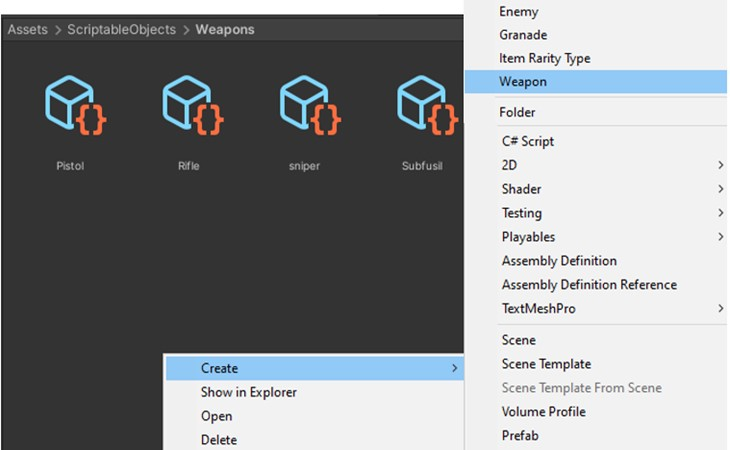
\includegraphics[scale=0.45]{img/NewWeapon.jpg}
    \caption{Crear un nuevo tipo de arma a través de un scriptableObject}
    \label{fig:CrearArmaScriptableObject}
    \end{figure}
    
    \item \textbf{\textit{Rellenar datos estáticos del arma}}
    Una vez creado el scriptableObject, se rellena con las propiedades, estadísticas y atributos del arma, como su daño, su alcance, su tiempo de recarga o las pistas de audio correspondientes que se crearon al principio (ver figura \ref{fig:PropiedadesEscopeta}).
    
    \begin{figure}[h]
    \centering
    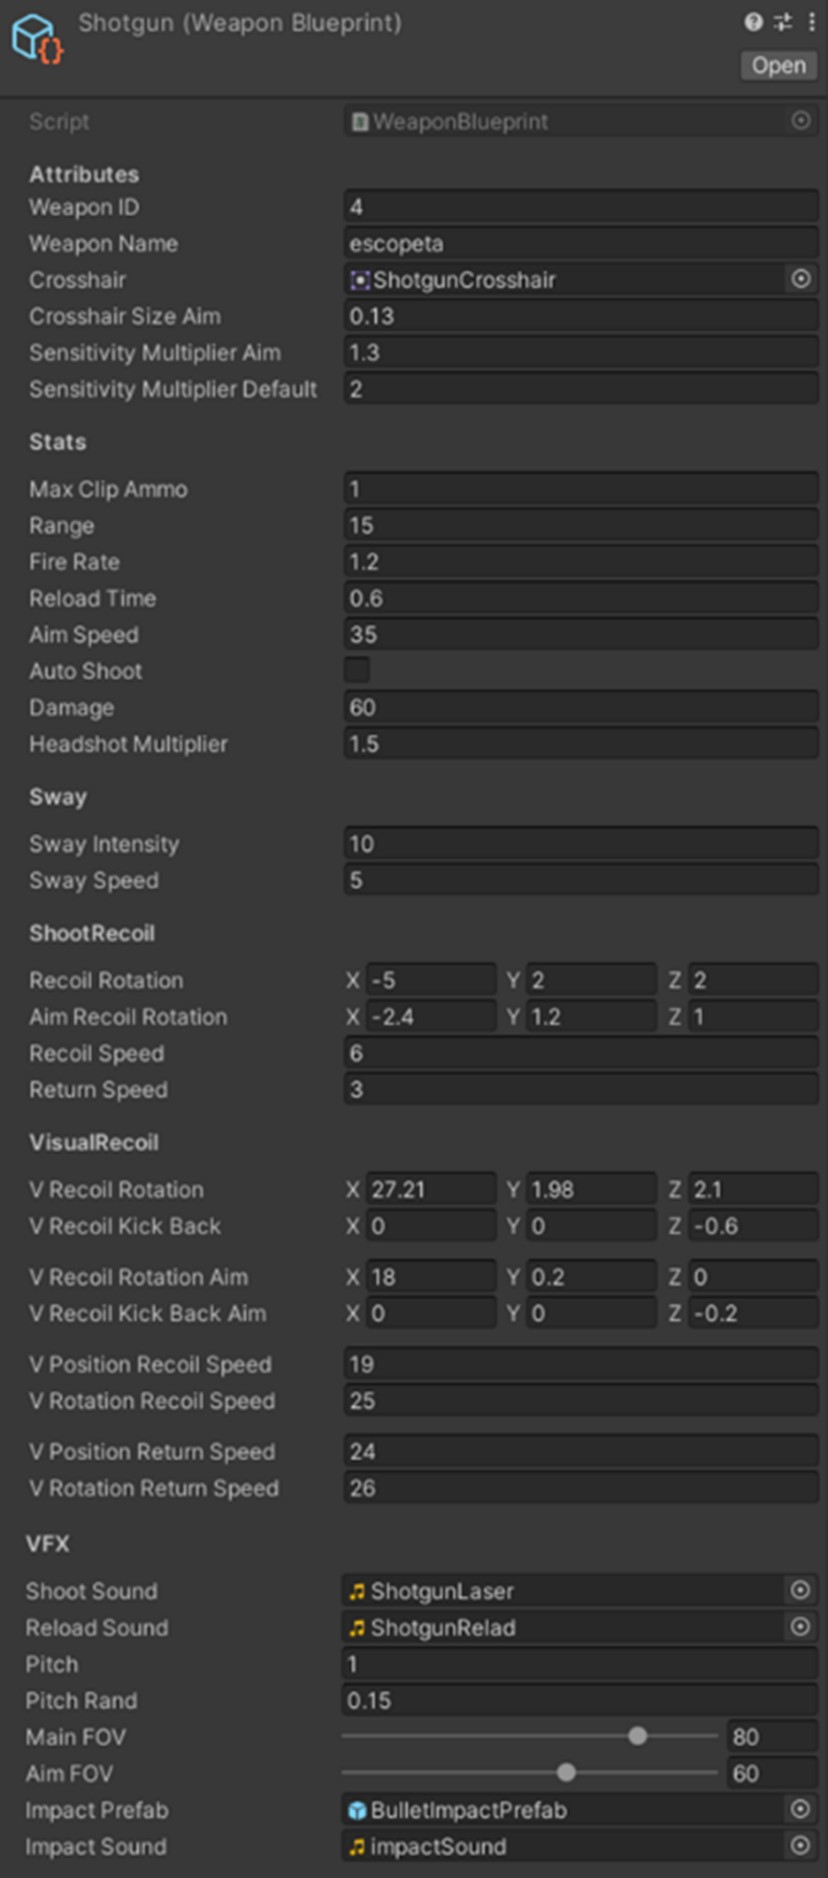
\includegraphics[scale=0.5]{img/ShotgunProperties.jpg}
    \caption{Propiedades y atributos de la escopeta}
    \label{fig:PropiedadesEscopeta}
    \end{figure}
    
    \item \textbf{\textit{Rellenar datos estáticos del arma}}
    Una vez creado el scriptableObject general del arma, hay que crear otros, esta vez a partir de la clase \textbf{\textit{ItemRarityBlueprint}}, para definir las propiedades y referencias de las distintas rarezas de la escopeta (ver figura \ref{fig:ScriptableObjectRarezas}). Entre ellas destacan: el modelo creado para representar cada rareza, el multiplicador de daño propio de cada una, la probabilidad que tiene un arma de dicha rareza de aparecer en cajas o cuándo se elimina a un enemigo.\\
    También contiene aspectos visuales, como los elementos que forman la etiqueta que aparece cuando el jugador mira hacia el arma, o el color y el icono del inventario cuando se equipa.
    
    \begin{figure}[h]
    \centering
    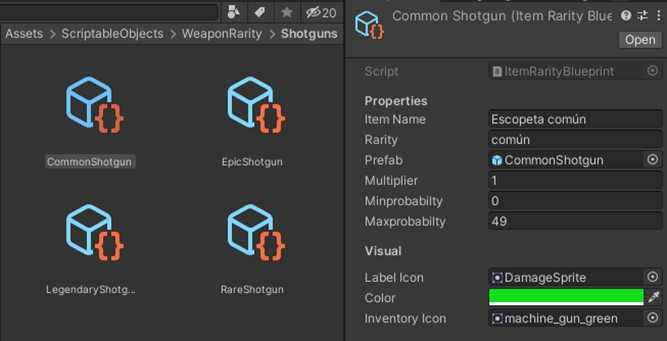
\includegraphics[scale=0.45]{img/CommonShotgunRarity.jpg}
    \caption{ScriptableObjects de las rarezas de la escopeta}
    \label{fig:ScriptableObjectRarezas}
    \end{figure}
    
    \item \textbf{\textit{Añadir el código necesario}}
     En el \textit{GameManager}, se deben añadir el conjunto de scriptableobjects de las rarezas para que pueda tener referencias a ellas al instanciar una escopeta. Asimisimo, en la clase \textit{Weapon}, propia de todas las armas, se debe incluir el caso de la escopeta al generar un arma, así como determinar su rareza desde el \textit{GamManager} en función de la probabilidad definida anteriormente para cada una de ellas (ver figuras \ref{fig:CodigoRarezasGameManager} y \ref{fig:CodigoRarezasWeapon}).
     
     \begin{figure}[h]
    \centering
    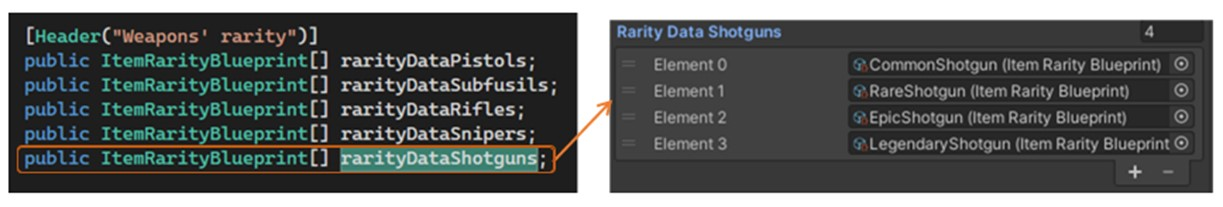
\includegraphics[scale=0.45]{img/ShotgunRarity.jpg}
    \caption{Código añadido en la clase \textit{GameManager} referente a las rarezas de la escopeta}
    \label{fig:CodigoRarezasGameManager}
    \end{figure}
    
    \begin{figure}[h]
    \centering
    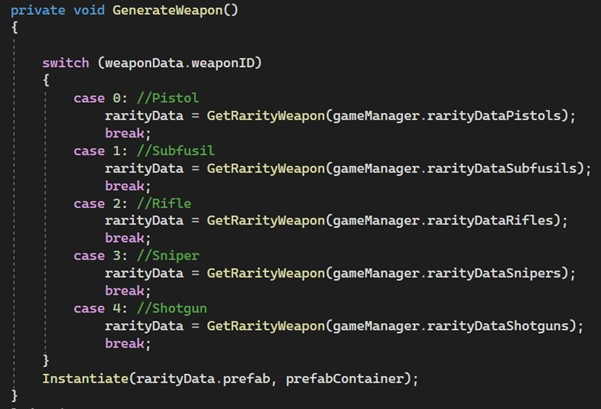
\includegraphics[scale=0.5]{img/GenerateWeapon.jpg}
    \caption{Código añadido a la clase \textit{Weapon} para crear la escopeta}
    \label{fig:CodigoRarezasWeapon}
    \end{figure}
    
     \item \textbf{\textit{Crear el Prefab de la escopeta}}
     El último paso es crear un \textbf{\textit{prefab}} que unifique todo lo anterior (ver figura \ref{fig:PrefabEscopeta}). Se le debe añadir el componente \textit{Weapon}, añadiendo el scriptableObject general de la escopeta en la variable ``WeaponData''.
     
     \begin{figure}[h]
    \centering
    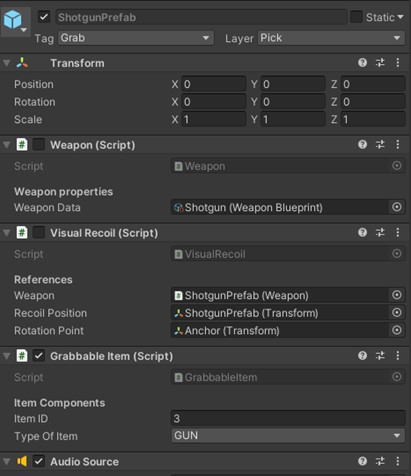
\includegraphics[scale=0.5]{img/ShotgunPrefab.jpg}
    \caption{Prefab de la escopeta}
    \label{fig:PrefabEscopeta}
    \end{figure}
    
\end{enumerate}
Este flujo de trabajo se puede extrapolar, aunque con salvedades en algunos pasos y con variaciones en ciertos componentes, al diseño y creación de otros datos y elementos del sistema, como, por ejemplo, el resto de armas, las granadas, los packs de ayuda o los enemigos.

\subsection{Diseño del inventario}
Una de las piezas centrales del videojuego es el inventario del personaje. A ojos del jugador, funcionará como una “mochila” en la que guardar objetos que se encuentre a su paso para poder usarlos de manera estratégica cuando considere conveniente.
Su diseño está configurado de la siguiente manera:

Se ha implementado la clase \textbf{\textit{InventorySlot}}, que representa cada uno de los espacios o compartimentos que tiene el inventario.

Internamente, cada slot funciona como una \textbf{pila de objetos} del tipo \textit{GrabbableItem}, es decir de los objetos que el jugador puede equiparse. La pila implementa las funciones propias de este tipo de estructuras, como las que permiten apilar (\textit{push}) un nuevo objeto, así como eliminar (\textit{pop}) o ver (\textit{peek}) el objeto de la cima de la pila, entre otras. Estas funciones están asociadas a ciertas acciones que hace el jugador durante la partida, como recoger o tirar un objeto.\\
También tiene otras funciones como, por ejemplo, comprobar, antes de apilar un objeto en un slot no vacío, que es compatible con el o los objetos que ya estén en la pila (\textbf{\textit{IsStackable}}).

Actualmente solo las granadas pueden apilarse en un mismo slot para así ahorrar espacio al jugador y que pueda llevar tantas granadas como se encuentre sin preocuparse de que se quede sin espacio en el inventario.

El inventario del jugador es una estructura de datos en forma de lista de slots, es decir, de instancias de la clase InventorySlot. En la figura \ref{fig:EstrucuraInventario} se puede ver la estructura general del inventario. Gestiona todos los objetos incluidos o potenciales de ser incluidos en él, controlando cuándo añadir o soltar un objeto del inventario, en qué slot debe ir cada objeto, o qué slot y, por tanto, qué objeto, debe estar activo en cada momento según el input del usuario.

\begin{figure}[h]
    \centering
    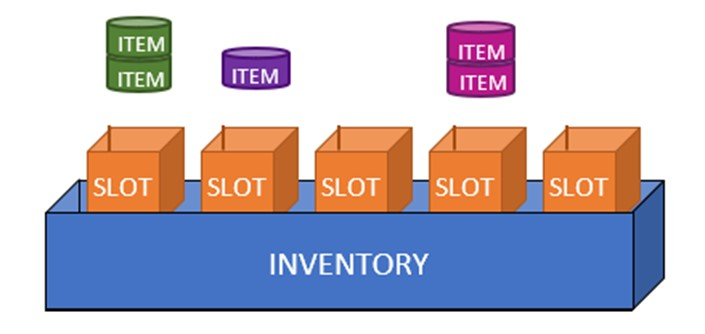
\includegraphics[scale=0.5]{img/InventoryScheme.jpg}
    \caption{Esquema de la estructura del inventario}
    \label{fig:EstrucuraInventario}
    \end{figure}
    
Además, como se ha mencionado en el apartado ``Events'' \ref{Events}, se utiliza la clase \textbf{\textit{InventoryVisuals}} para gestionar toda la parte audiovisual del inventario, manteniéndola separada de la lógica real.\\
Se encarga de mostrar por medio de una interfaz, los espacios del inventario, a través de imágenes en forma romboidal.\\
Cada uno de ellos tendrá una imagen de la clase de objetos que contiene dicho espacio en la parte lógica en caso de no estar vacío. Asimismo, pintará tanto el borde como el fondo del espacio de un color según el tipo o la rareza del objeto, y hará que el espacio o slot activo sea más grande que el resto para que el jugador sepa qué arma o granada puede usar en cada momento (ver figura \ref{fig:InterfazInventario}). Todo ello acompañado de efectos de sonido cuando el jugador cambie de objeto activo, lo tire al suelo o recoja alguno del suelo.

\begin{figure}[h]
    \centering
    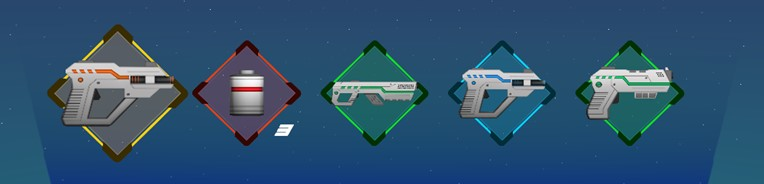
\includegraphics[scale=0.55]{img/InventoryInterface.jpg}
    \caption{Interfaz del inventario en uso}
    \label{fig:InterfazInventario}
    \end{figure}
    
De esta forma se consigue diseñar una estructura de datos que pueda gestionar adecuadamente todos los objetos que el jugador tenga equipados. Así, a un alto nivel, será sencillo y natural para el jugador recoger, tirar, usar o cambiar de arma y que haya un feedback audiovisual claro de estas acciones (ver diagrama de clases en la figura \ref{fig:InventarioUML})

\begin{figure}[h]
    \centering
    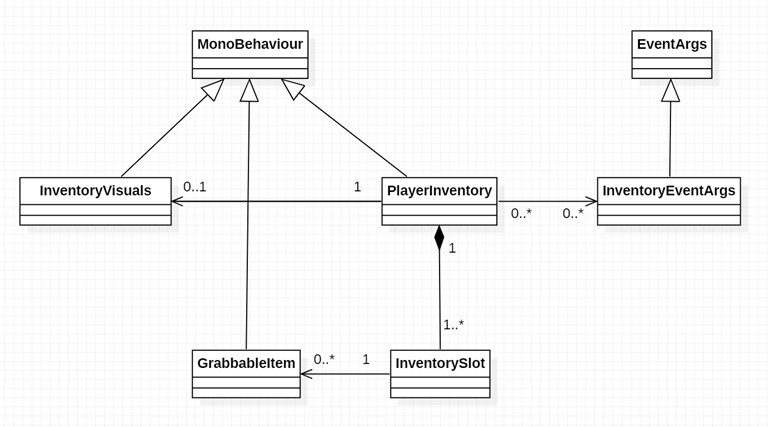
\includegraphics[scale=0.45]{img/InventoryClassDiagram.jpg}
    \caption{Diagrama de clases del inventario del jugador}
    \label{fig:InventarioUML}
    \end{figure}
    
\subsection{Diseño de interfaces}
El diseño de las interfaces de la aplicación es una parte fundamental del proyecto para asegurar el buen uso del videojuego, además de ser un elemento estético importante que conecta visualmente al resto de elementos. Es la forma en la que usuario y sistema se comunican durante gran parte del tiempo y, por ello, la experiencia de usuario al navegar o interactuar con cualquiera de las pantallas debe ser fluida, intuitiva y clara.

Se han utilizado varios elementos para conseguir esta facilidad de uso de las interfaces. Por ejemplo, se han escogido colores vivos, tipografías con un estilo futurista pero fáciles de leer, con un tamaño adecuado y botones grandes y descriptivos.

Se ha intentado mantener un cierto minimalismo en la composición visual, así como una armonía estética, haciendo uso de colores complementarios, degradados, y contrastando los elementos importantes, como el texto y los botones con el fondo. También se ha intentado dar énfasis a algunos elementos utilizando el color o el tamaño, como se puede apreciar (ver figura \ref{fig:InterfacesManuRegistro}), por ejemplo, en el menú principal, donde el botón de ``jugar'' es más grande que el resto para darle una importancia mayor y el botón de ``salir'' tiene un color rojizo para indicar alerta.

\begin{figure}[h]
    \centering
    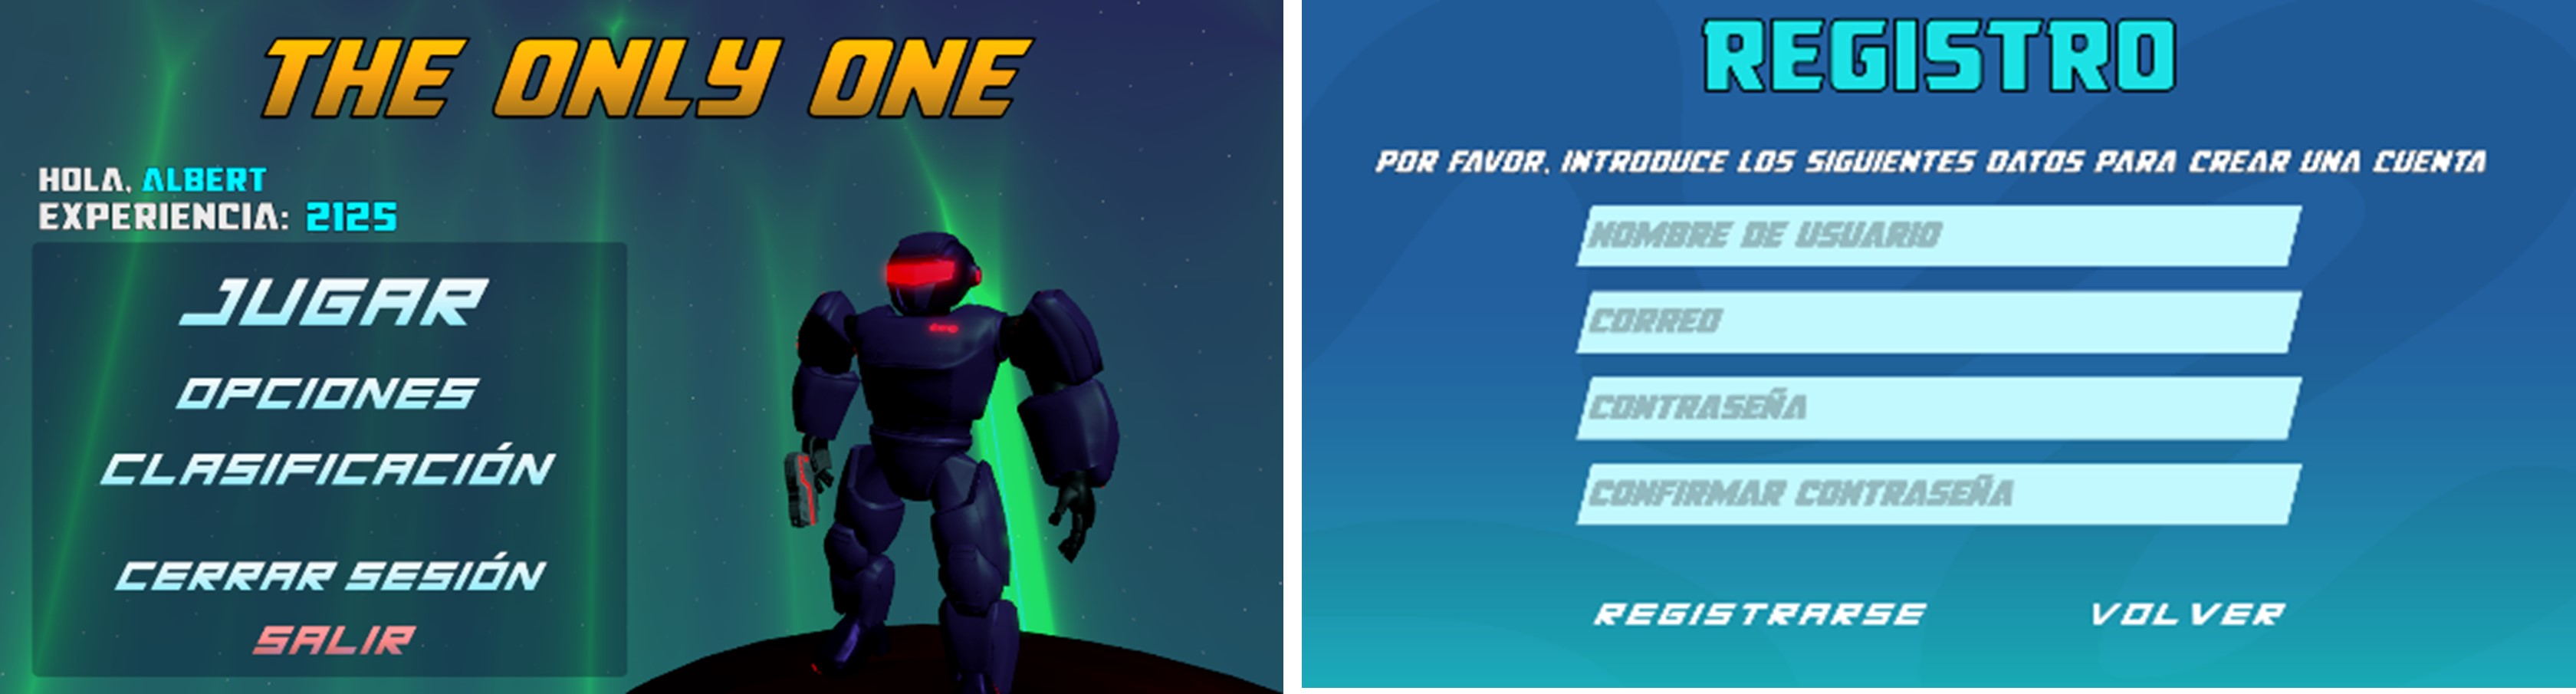
\includegraphics[scale=0.45]{img/Interfaces.jpg}
    \caption{Interfaces del menú principal y de registro}
    \label{fig:InterfacesManuRegistro}
    \end{figure}
    
Hay que mencionar también la existencia de una \textbf{pantalla de carga} que se muestra en las transiciones entre escenas, que es cuando más tiempo toma la aplicación para cargar los elementos. De esta forma, el jugador recibe en todo momento algún tipo de feedback del estado de la aplicación, evitando así que piense que la aplicación se ha congelado, está en algún estado de error al ver una pantalla negra o que no responde a su input.

En ella se puede ver la nube tóxica desde lejos a modo de fondo, así como el título del videojuego, junto a un pequeño eslogan. También se incluye una rueda de carga que gira continuamente, y la palabra ``cargando…'' para informar al usuario de que la escena está en proceso de carga (ver figura \ref{fig:PantallaDeCarga}).

\begin{figure}[h]
    \centering
    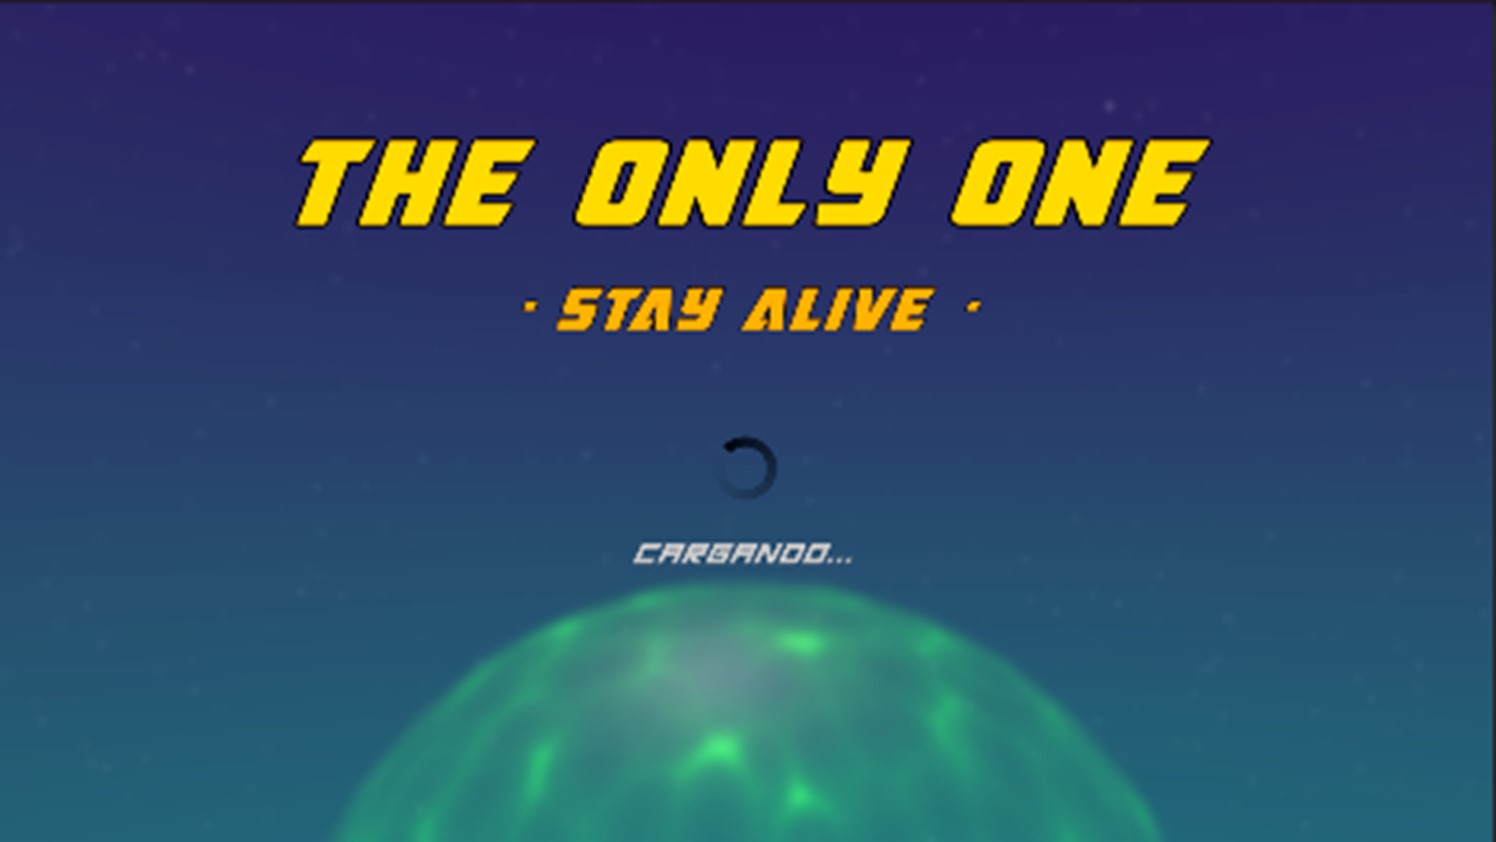
\includegraphics[scale=0.45]{img/LoadingScreen.jpg}
    \caption{Pantalla de carga del videojuego}
    \label{fig:PantallaDeCarga}
    \end{figure}
    
Finalmente, para el diseño del \textbf{logo del videojuego} se ha utilizado el software de edición de vectores llamado Illustrator, y se han querido reflejar en él algunos de los elementos del videojuego, como la cabeza de los enemigos, que además sirve como letra “O” para completar el título del videojuego o la corona que simboliza la victoria. Todo esto enmarcado en un círculo que simboliza la zona segura del mapa (ver figura \ref{fig:Logo}).

\begin{figure}[h]
    \centering
    
\includegraphics[scale=0.45]{img/Logo_TheOnlyOne.png}
    \caption{Logo del videojuego ``The Only One''}
    \label{fig:Logo}
    \end{figure}

\section{Diseño procedimental}
Una vez visto cómo se han diseñado los datos principales de la aplicación para poder construirla, se analizarán ahora los flujos de ejecución de los datos descritos en tiempo de ejecución para entender de qué manera funcionan los procesos y los estados de los componentes del videojuego.

\subsection{Flujo de autenticación e interacción con la base de datos}
La autenticación de un usuario de la aplicación es un proceso que integra varios pasos, entre los que destaca la interacción con la base de datos conectada a la aplicación.

El sistema hará operaciones de lectura y escritura en la base de datos en función de la información que requiera actualizar o solicitar.

En la figura \ref{fig:DiagramaBBDD} se puede ver, a grandes rasgos, el conjunto de secuencias de datos que hay entre el usuario, la aplicación y la base de datos, desde que el usuario se registra hasta que termina una partida y puede ver su experiencia reflejada en la interfaz del menú principal. Se ha elaborado el diagrama sobre dicha secuencia de acciones porque incluye todas las peticiones y respuestas posibles con la base de datos.

\begin{figure}[h]
    \centering
    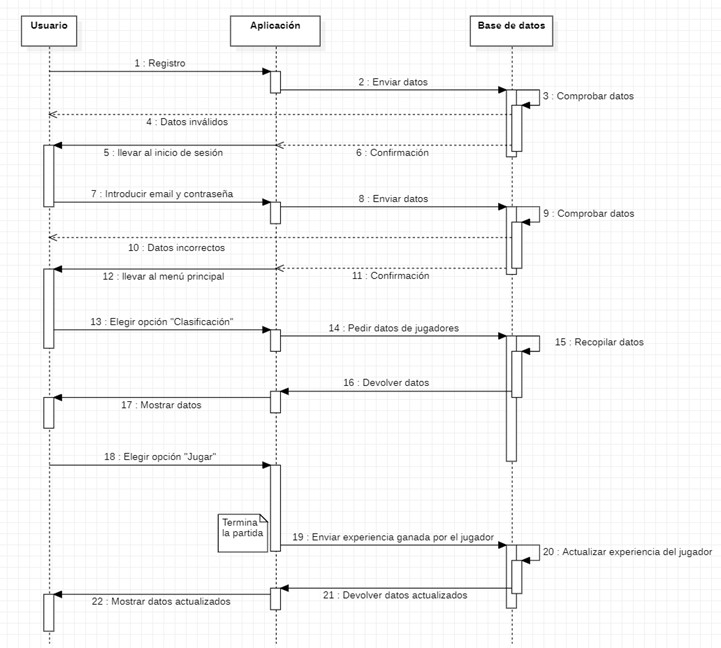
\includegraphics[scale=0.55]{img/DatabaseUsageFlowchart.jpg}
    \caption{Diagrama de secuencia del uso de la base de datos}
    \label{fig:DiagramaBBDD}
    \end{figure}

\subsection{Estados del jugador}
El jugador, a lo largo de la partida, puede pasar por diferentes estados según las situaciones que ocurran o las acciones que tome el usuario como input. En la figura \ref{fig:EstadosJugador} se reflejan los distintos estados con relación a su \textbf{movimiento}.\\
Cabe destacar que, desde cualquiera de ellos, se puede recibir daño, morir o ganar la partida. Son estados que no se incluyen en el diagrama por su trivialidad.

\begin{figure}[h]
    \centering
    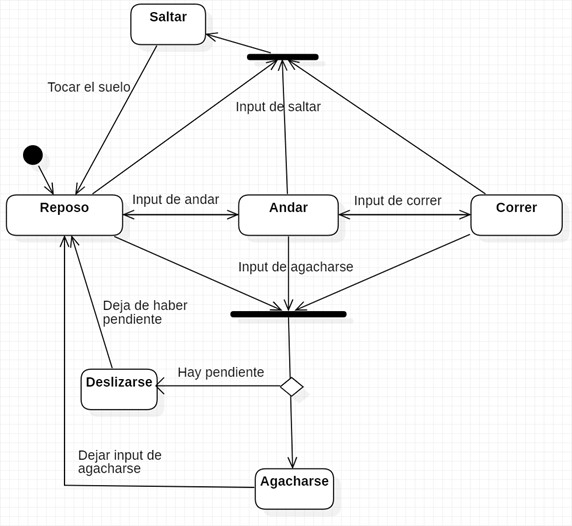
\includegraphics[scale=0.5]{img/PlayerStatesDiagram.jpg}
    \caption{Diagrama de estados del jugador}
    \label{fig:EstadosJugador}
    \end{figure}

\subsection{Salud del jugador}
Para entender el funcionamiento del sistema de salud del jugador, se representa en los siguientes diagramas el flujo de ejecución de sus diferentes componentes (ver figuras \ref{fig:DiagramaCuracion}, \ref{fig:DiagramaArmadura} y \ref{fig:DiagramaDaño}).

\begin{figure}[h]
    \centering
    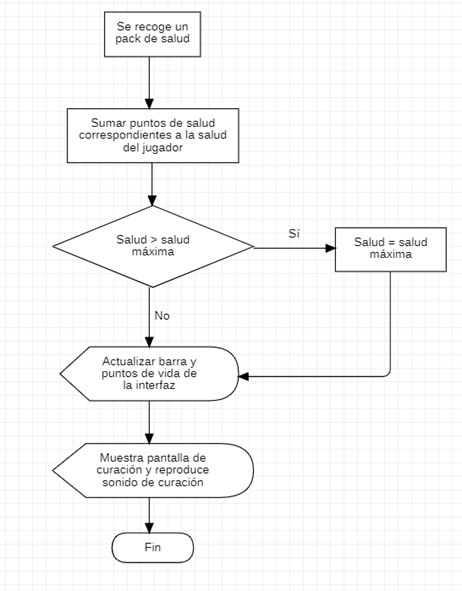
\includegraphics[scale=0.5]{img/HealingFlowchart.jpg}
    \caption{Diagrama de flujo de curación}
    \label{fig:DiagramaCuracion}
    \end{figure}
    
\begin{figure}[h]
    \centering
    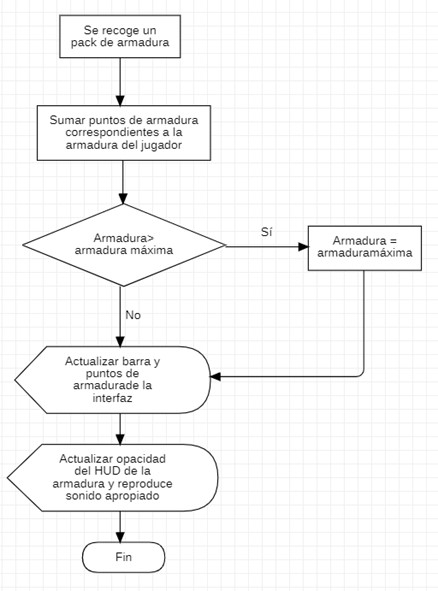
\includegraphics[scale=0.5]{img/ArmorRecoveryFlowchart.jpg}
    \caption{Diagrama de flujo de recuperación de armadura}
    \label{fig:DiagramaArmadura}
    \end{figure}
    
\begin{figure}[h]
    \centering
    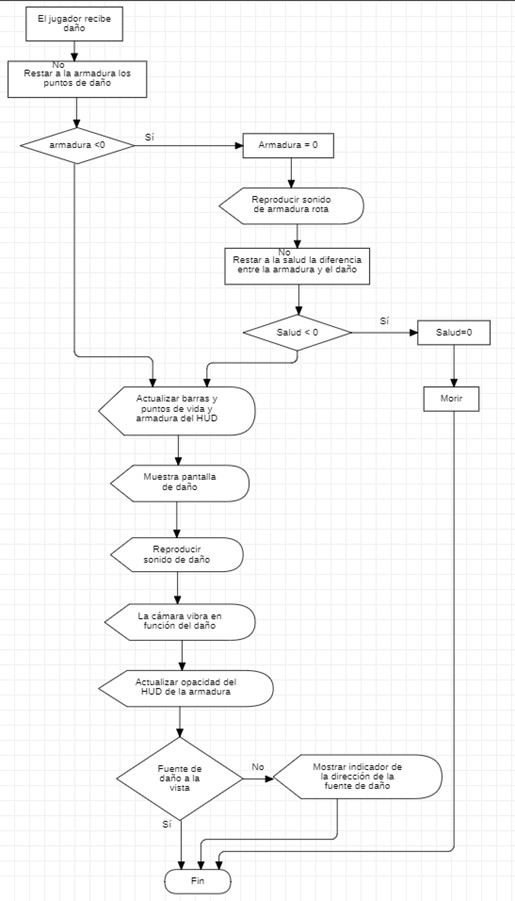
\includegraphics[scale=0.5]{img/DamageFlowchart.jpg}
    \caption{Diagrama de flujo de recibir daño}
    \label{fig:DiagramaDaño}
    \end{figure}

\subsection{Estados del enemigo}
Para generar un comportamiento verosímil de los enemigos, se ha desarrollado un sistema que trata de simular el comportamiento real de un jugador.  De acuerdo con esto, su funcionamiento se ha diseñado como una \textbf{máquina de estados} en la que, dependiendo en qué condición se encuentre, podrá realizar unas acciones u otras. Estas situaciones llevarán al enemigo a encontrarse en diferentes estados a medida que avanza el transcurso de la partida, todo ello en tiempo real.

En la figura \ref{fig:DiagramaEnemigo} se muestra el diagrama que representa los estados y las condiciones para pasar de unos a otros (los estados en azul son en movimiento, mientras que los naranjas son estáticos):

\begin{figure}[h]
    \centering
    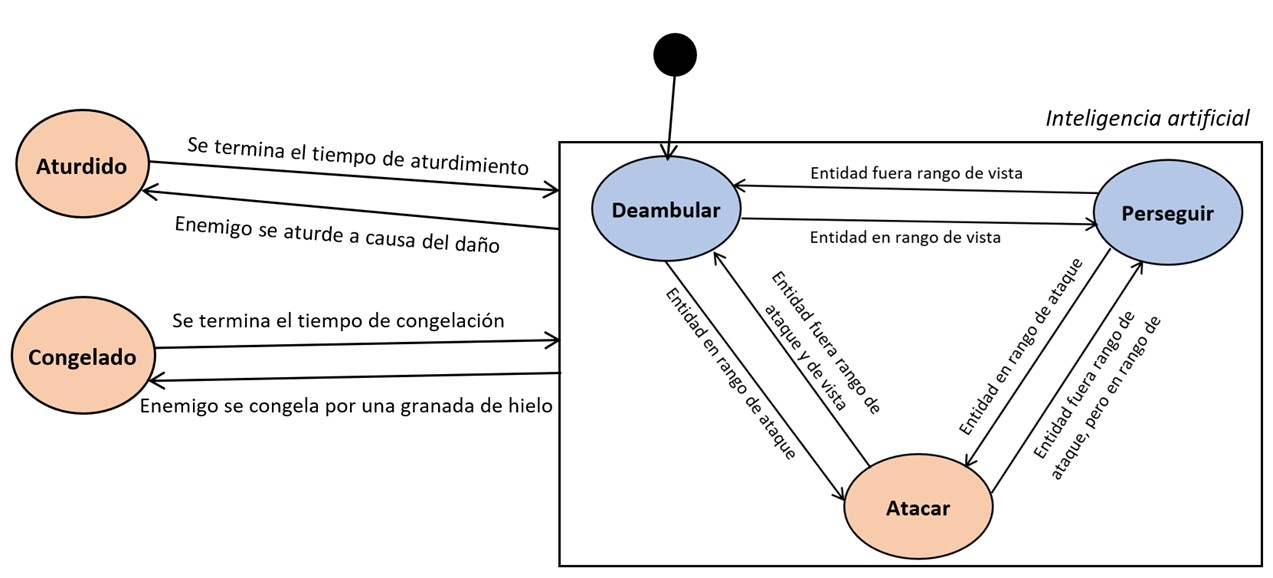
\includegraphics[scale=0.45]{img/EnemyStates.jpg}
    \caption{Diagrama de estados del enemigo}
    \label{fig:DiagramaEnemigo}
    \end{figure}
    
\subsection{Añadir un objeto al inventario}
Uno de los aspectos a destacar del proyecto es el modo en que funciona el inventario del jugador. Para visualizar el procedimiento que se sigue a la hora de coger un objeto y hacer que se asigne de manera correcta y ordenada en el inventario, se muestra a modo de esquema, en la figura \ref{fig:DiagramaRecogerObjeto}, un diagrama donde se visualizan las principales acciones y comprobaciones que ocurren, desde que el jugador pulsa la tecla de recoger el objeto hasta que lo tiene equipado, listo para usarse, incluyendo feedback visual.

\begin{figure}[h]
    \centering
    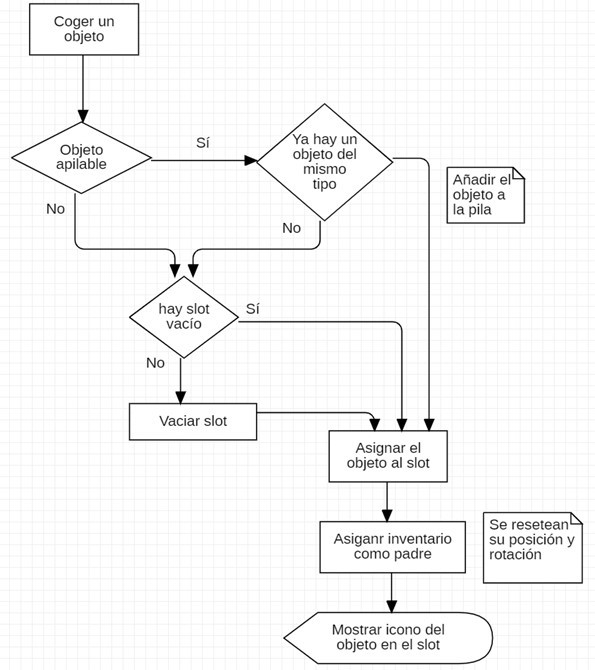
\includegraphics[scale=0.5]{img/PickingObjectFlowchart.jpg}
    \caption{Diagrama de flujo de recoger un objeto}
    \label{fig:DiagramaRecogerObjeto}
    \end{figure}

\subsection{Flujo de escenas e interfaces}
Con el objetivo de visualizar mejor todas las interfaces que componen el videojuego, se ha creado un esquema (ver figura \ref{fig:DiagramaPantallas}) a modo de diagrama que representa el flujo de ejecución de la aplicación a través de la interconexión entre ellas.

\begin{figure}[h]
    \centering
    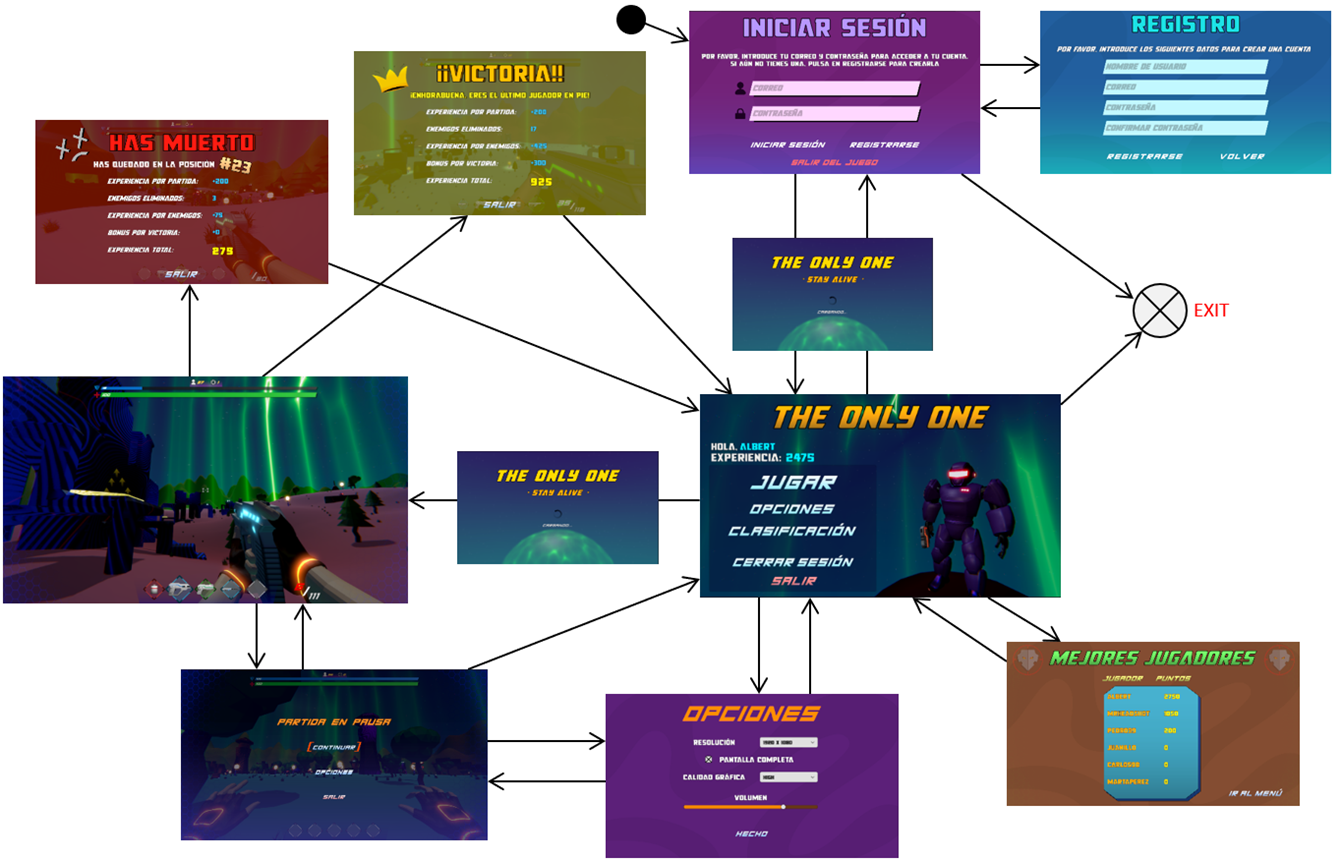
\includegraphics[scale=0.4]{img/ScreenFlowChart.png}
    \caption{Diagrama de flujo entre pantallas}
    \label{fig:DiagramaPantallas}
    \end{figure}
    
\section{Diseño arquitectónico}
En este apartado se analizará la estructura general de la aplicación como software creado dentro de un motor de videojuegos, así como el modo en el que se relaciona con otras entidades, como la base de datos, las diferentes librerías que utiliza o los paquetes usados en la aplicación.

El controlador que gestiona todos los paquetes de la aplicación es el llamadado \textbf{\textit{Package Manager}} \cite{doc:PackageManager} o Controlador de paquetes. Es un contenedor proporcionado por Unity para almacenar varios tipos de archivos y características, como librerías, frameworks, o dependencias del proyecto.

Algunos de los paquetes internos que utiliza este proyecto son los que se listan en la  figura \ref{fig:Paquetes internos}:
\begin{figure}[h]
    \centering
    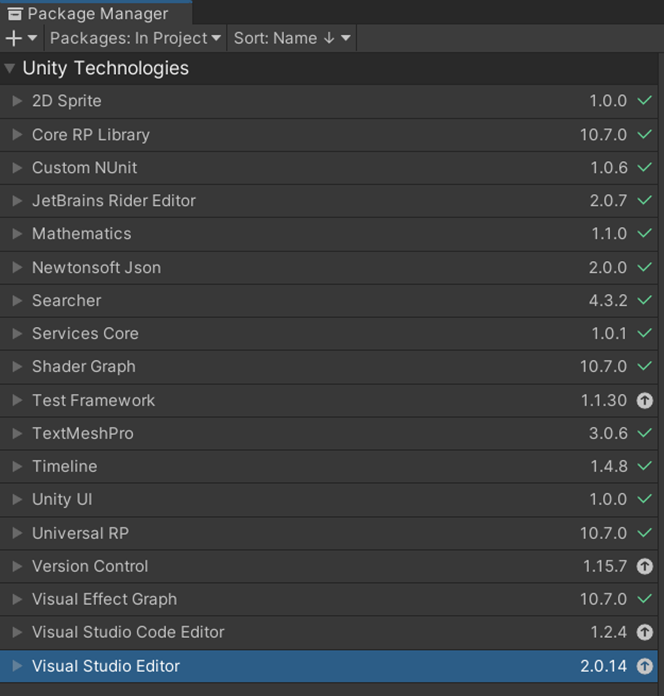
\includegraphics[scale=0.45]{img/PackagesUnity.png}
    \caption{Paquetes internos de Unity en el proyecto}
    \label{fig:Paquetes internos}
    \end{figure}
    
Por ejemplo, el paquete ``Shader Graph'' añade a Unity un editor visual de shaders, que se ha utilizado para crear algunos de los shaders del proyecto, como el de la nube tóxica, el rastro de las granadas o el cielo. Otro paquete digno de mencionar es \textit{TextMeshPro}. Este paquete incluye todo un conjunto de herramientas para crear textos de calidad en el proyecto. De hecho, todos los textos que se pueden ver en la aplicación están creados con esta librería.

Algunos paquetes ofrecen funcionalidades añadidas y opcionales, como los descritos anteriormente, pero otros son fundamentales para que la aplicación funcione correctamente a nivel interno, como el paquete de Servicios \textit{Services Core}, que define los componentes comunes de los \textit{Game Services Packages}.

Existen otro tipo de paquetes externos, añadidos por el desarrollador, que se han importado al proyecto desde la \textit{Unity Asset Store}. Estos son:
\begin{itemize}
    \item \textbf{2D Sci-Fi Weapon Pack}: paquete de imágenes destinadas a representar los iconos de las armas y las granadas en el inventario.
    \item \textbf{Sci-Fi Weapons Pack}: paquete de modelos 3D de las armas base utilizadas, así como sus texturas.
    \item \textbf{Quick Outline}: librería utilizada para colorear el borde de los objetos cuando se puede interactuar con ellos.
    \item \textbf{Robot Soldier}: modelo 3D del robot utilizado como enemigo.
    \item \textbf{Lean Tween}: librería para animar elementos de la interfaz, empleada cuando el jugador mata a un enemigo y cuando aparece la pantalla del resumen de la experiencia ganada al final de la partida.
\end{itemize}
Cuando Unity carga un proyecto, el Package Manager lee el \textbf{\textit{Project manifest}} para comprobar una lista de paquetes y dependencias que debe recuperar y cargar. Es un archivo en formato JSON que se actualiza cuando, por ejemplo, el desarrollador instala o desinstala un paquete externo.

El archivo \textit{manifest.json}, al momento de compilar la aplicación final, se ve como en la figura \ref{fig:ManifestJSON}:

\begin{figure}[h]
    \centering
    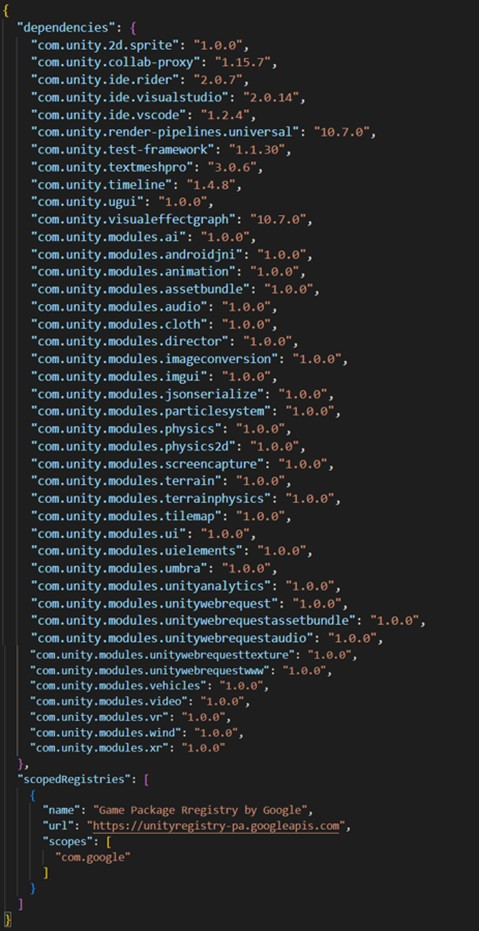
\includegraphics[scale=0.45]{img/Manifestjson.jpg}
    \caption{Archivo manifest.json}
    \label{fig:ManifestJSON}
    \end{figure}
    
La forma en la que Unity integra los paquetes es la siguiente (ver figura \ref{fig:FlujoPaquetes}):

\begin{enumerate}
    \item Al abrir un proyecto, el package manager lee el manifest.json para saber qué paquetes cargar.
    \item Envía una petición al package registry server o servidor de registro de paquetes por cada paquete que aparezca como dependencia en el archivo manifest
    \item El registro de paquetes envía la información solicitada de vuelta al package manager.
    \item El package manager instala los paquetes en el proyecto.
\end{enumerate}

\begin{figure}[h]
    \centering
    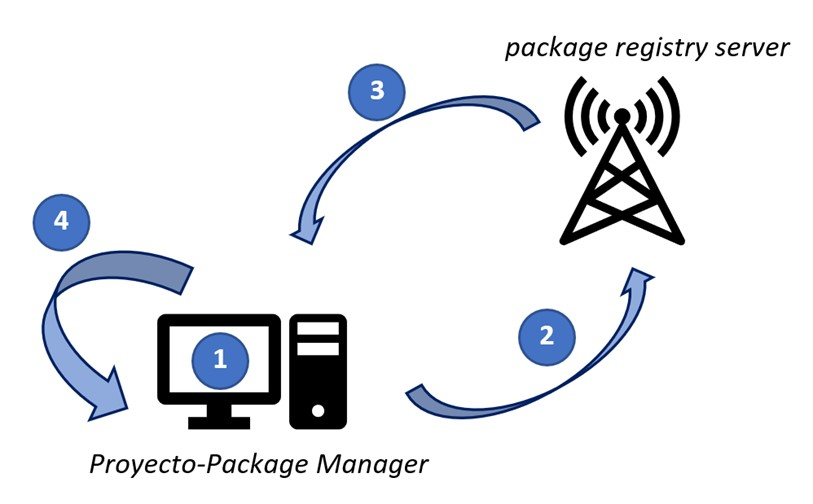
\includegraphics[scale=0.45]{img/PackageManagerFlowchart.jpg}
    \caption{Flujo de peticiones de paquetes}
    \label{fig:FlujoPaquetes}
    \end{figure}

Cuando se instala un paquete desde el \textit{Package Manager}, realmente se están añadiendo dependencias al archivo manifest.json. Con ello se especifica la versión particular del paquete que se necesita para que el proyecto funcione como se espera. Estas dependencias que aparecen en el Project manifest se denominan dependencias directas.

Sin embargo, los paquetes puede que necesiten de otros paquetes para que funcionen. Estas serían las dependencias indirectas, y se deberían añadir de manera automática al instalar el paquete deseado. Si no lo hacen, se tienen que resolver esas dependencias manualmente o refrescando la importación.

Cuando el \textit{Package Manager} resuelve con éxito todas las versiones adecuadas de las dependencias, se guarda esta resolución en un archivo llamado \textbf{\textit{packages-lock.json}}. Así se asegura la consistencia y la velocidad de carga de las dependencias cuando se carguen en el proyecto. En la figura \ref{fig:PaqueteLock} se puede ver un fragmento de su contenido:
\begin{figure}[h]
    \centering
    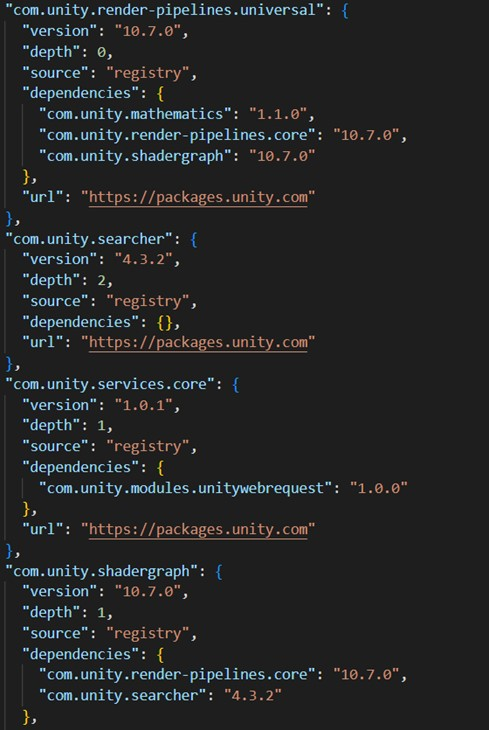
\includegraphics[scale=0.45]{img/Packages-lockJSON.jpg}
    \caption{Fragmento del archivo \textit{Packages-lock.json}}
    \label{fig:PaqueteLock}
    \end{figure}
Respecto a la base de datos a la que se conecta la aplicación, la estructura que sigue la conexión y el envío de datos se entiende mejor si se conoce cómo se ha implementado y cuál es su configuración.

Los pasos seguidos para integrar y conectar la aplicación a la base de datos en tiempo real de Firebase y para implementar la autenticación de usuarios fueron los siguientes:
\begin{enumerate}
    \item \textbf{Crear un proyecto de Firebase}: Un proyecto de Firebase es el contenedor de todos los servicios y recursos asociados a la aplicación a la que se conecta. Este proyecto, llamado ``TheOnlyOne'', por el momento, solamente utiliza los servicios de ``Authentication'' y ``Realtime Database'' para cubrir las necesidades requeridas (ver figura \ref{fig:JerarquíaFirebase}).
    
    \begin{figure}[h]
    \centering
    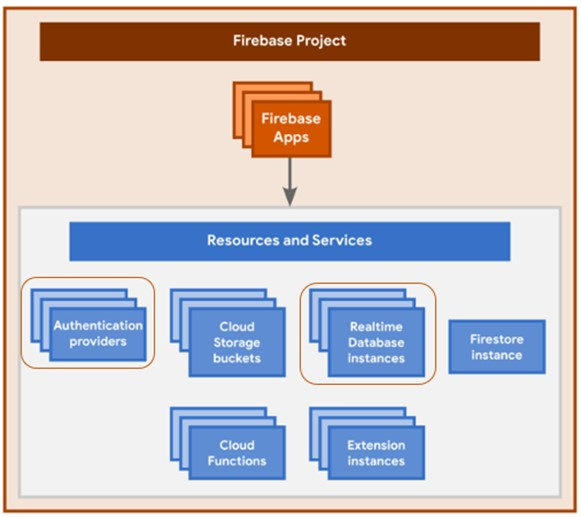
\includegraphics[scale=0.45]{img/HierarchyFirebaseProject.jpg}
    \caption{Esquema de la jerarquía de un proyecto de Firebase}
    \label{fig:JerarquíaFirebase}
    \end{figure}
    
    \item \textbf{Registrar la aplicación con Firebase}: En este paso se asocia cada versión que se vaya a compilar de la aplicación (Android, iOS…) al proyecto de Firebase, añadiendo el ID de del proyecto de Unity. En este caso, el ID de la aplicación para la plataforma Android es ``com.AlbertoFuente.TheOnlyOne''. 
    
    Si bien la aplicación no se ejecutará en Android, es la opción que se debe marcar para crear un proyecto de escritorio.
     \item \textbf{Agregar los archivos de configuración de Firebase}. En este paso se debe descargar un archivo llamado \textbf{\textit{google-services.json}} y añadirlo a la carpeta de assets del proyecto en Unity.
     
     Después se debe agregar el SDK de Firebase para Unity. Concretamente, se importan a Unity los paquetes que sean relevantes para el proyecto, así como las dependencias de estos para que puedan funcionar. En este caso, se añaden “FirebaseDatabase.unitypackage” para la configuración de la base de datos, y “FirebaseAuth.unitypackage” para la autenticación de usuarios. Antes de importar estos paquetes se debe comprobar qué versión de la librería .NET utiliza el proyecto, que en este caso es .NET 4.
    \item \textbf{Resolver las dependencias} de los paquetes importados desde el gestor de dependencias de Unity.
    \item \textbf{Crear la Base de datos}. En la consola de Firebase, crear la base de datos que utilizará el proyecto
    \item \textbf{Crear un método de autenticación de usuarios}: En la consola de Firebase, elegir el modo de acceso que se desea que utilicen los usuarios de la aplicación. En este proyecto se utiliza correo y contraseña como procedimiento de autenticación.
\end{enumerate}
Siguiendo todos estos pasos, ya estaría lista la configuración inicial de la base de datos y el método de autenticación de los usuarios para acceder a ella.

Como se puede observar en la figura \ref{fig:ManifestJSON}, que forma parte del archivo manifest.json, además de las dependencias, se puede ver un apartado llamado \textbf{\textit{Scoped Registries}}. Este tipo especial de registros permiten a Unity comunicar al package manager dónde se encuentra cada servidor de registro de paquetes. De esta forma, el usuario puede acceder a grandes colecciones de paquetes al mismo tiempo.

Al integrar la base de datos de Firebase con el proyecto de Unity, se instala automáticamente un Scoped Registry asociado a la API de Google para que la conexión con Firebase pueda producirse adecuadamente y se acceda a todos los paquetes necesarios (ver figura \ref{fig:ScopedRegistry}).
\begin{figure}[h]
    \centering
    \includegraphics[scale=0.45]{img/ScopedRegistry .jpg}
    \caption{\textit{Scoped registry} de Google}
    \label{fig:ScopedRegistry}
    \end{figure}


